\documentclass[a4paper, 11pt]{article}
\usepackage[utf8]{inputenc}
\usepackage[lmargin=3cm]{geometry}
\usepackage{amssymb}
\usepackage{verbatim}

\hyphenation{FORTRAN NEKBONE}

%Inlucde common settings

% ****************************************************************************************************
% Loading some handy packages
% ****************************************************************************************************
\usepackage{hyperref}
\usepackage[english]{babel}
\usepackage{graphicx}
\usepackage{fancyhdr}
\usepackage{datetime}
\usepackage{listings}
\usepackage{amsmath}
\usepackage{multirow}
\usepackage{array}
\usepackage{color}
\usepackage[square,numbers]{natbib}

\usepackage{algorithm}
\usepackage{algorithmic}
\renewcommand{\algorithmicrequire}{\textbf{Input:}}
\renewcommand{\algorithmicensure}{\textbf{Output:}}


%\usepackage[textsize=tiny,color=blue!2,textwidth=0cm]{todonotes}


%****************************************************************************************************
% Fine-tuning and further settings
% ****************************************************************************************************

\hyphenation{ VAMPIR KOJAK time-stamp }

%\textwidth=17cm

%\textheight=22cm

\setlength{\unitlength}{0.5cm}

\setlength{\parindent}{0.0cm}

\setlength{\parskip}{1.0ex}

%\addtolength{\leftargin}{-1cm}

\linespread{1.0}

\raggedbottom \sloppy

%\addtolength{\evensidemargin}{1cm}

%\addtolength{\oddsidemargin}{-2cm}

\addtolength{\topmargin}{-0.5cm}

% date formatting
\renewcommand{\dateseparator}{.}


%****************************************************************************************************
% Header and Footer
% ****************************************************************************************************

\pagestyle{fancy}
\lhead{AutoTune}
\chead{} % Define this in your document to Deliverable Dx.y
\rhead{\date}
\cfoot{} % important (eliminated standard page number on footer)
\rfoot{\thepage}
\renewcommand{\headrulewidth}{0pt}

%****************************************************************************************************
% Some TODO's commands and settings
% ****************************************************************************************************
% own comments and commands for all authors:
%\newcommand{\AuthorsList}{% NOTE: no spaces after comma
%MG,% Michael Gerndt
%IC,% Isaias Compres
%MS,% Martin Sandrieser
%LM,% Laurent Morin
%CG,% Carla Guillen
%EC,% Eduardo Caesar
%AB}% Anca Berariu

% Anca Berariu (AB)
%\newcommand{\mytodoAB}[2][]{\todo[color=blue!2,noline, #1]{\textbf{TODO[AB]:} #2}}
%\newcommand{\mycommentAB}[2][]{\todo[color=yellow!25,line, #1]{\textbf{Comment[AB]:} #2}}
%\newcommand{\myfixmeAB}[2][]{\todo[color=red!5,noline, #1]{\textbf{FIXME[AB]:} #2}}
% et.al. ........
% ...............
% ...............

%default commands
%\newcommand{\mytodo}[2][]{\todo[color=blue!2,noline, #1]{\textbf{TODO:} #2}}
%\newcommand{\mycomment}[2][]{\todo[color=yellow!25,line, #1]{\textbf{Comment:} #2}}
%\newcommand{\myfixme}[2][]{\todo[color=red!5,line, #1]{\textbf{FIXME:} #2}}

%command for adding subsubsub section using \paragraph
\usepackage{titlesec}
\setcounter{secnumdepth}{4}

\titleformat{\paragraph}
{\normalfont\normalsize\bfseries}{\theparagraph}{1em}{}
\titlespacing*{\paragraph}
{0pt}{3.25ex plus 1ex minus .2ex}{1.5ex plus .2ex}


\newenvironment{code}%
{
\addtolength{\leftskip}{0.5cm}}%
{

}

\begin{document}

\title{
\includegraphics[width=4cm]{./images/Ptf_LogoBlau}\\ \vspace{1cm}
\textsf{\bf \huge Best Practice Guide }\\
       \normalsize PTF Version: 1.1\\
       }
\author{AutoTune Partners}
\date{14.04.2015}
\maketitle
\newpage
\tableofcontents

\newpage
\section{Introduction}

\label{sec:intro}
The Periscope Tuning Framework (PTF) is an extension to the existing performance analysis tool Periscope. PTF makes it possible to use profiling information gathered by Periscope and employ it for automatically tuning software applications. 

There are five tuning plugins available as part of PTF, which target different tuning problems/techniques and which can be used to improve the performance and energy efficiency of a given application with one or more tuning techniques.

PTF and its associated tuning plugins provide many features to aid users in their effective exploitation. It is therefore useful to understand these features and techniques so as to be able to extract maximum benefit out of PTF. 

This Best Practice Guide provides various ways to use each plugin more effectively as well as obtain tuning results more efficiently. In Section 2 of this guide, we explain how PTF fits into the overall tuning lifecycle. In Section 3, we provide several generic best practices applicable for all the plugins as well as the steps required for manual instrumentation. Finally, in Section 4, best practices specific to each of the separate plugins are provided.

\clearpage

\section{PTF in the Tuning Cycle}
\label{sec:chapter2}
The typical approach to software application tuning begins with selecting the baseline which is a version of the application used as a reference in all the further tuning steps. The process subsequently involves profiling the application to identify the performance bottlenecks of the application.  Once identified, these bottlenecks are analyzed and a particular bottleneck is selected for tuning with the aim of improving the performance (e.g., time to solution) of the application. The tuning technique to be used on the bottleneck is identified and applied to the application and the tuning cycle begins again.

\begin{figure}[H]
\centering
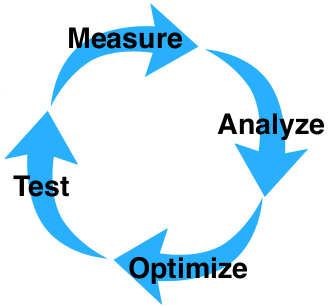
\includegraphics[scale=.6]{../BPG/images/tuning_cycle.png}
\caption{Application tuning cycle}
\label{fig:tuning_cycle}
\end{figure}

When implemented manually, the tuning process is iterative, cumbersome and often very time consuming. PTF provides tuning plugins which can perform the application tuning automatically and remove this burden of manual tuning from the application developer. The tuning plugins explore the available tuning search space, evaluate different tuning scenarios and return the end results to the users without any human interventions. Along with automatic evaluation, PTF provides smarter ways to explore possible search combinations using various search strategies. For example, in particular cases, PTF can evaluate the optimal combination without complete execution of the application which reduces the tuning times drastically. 

Use of automatic tuning contributes towards the overall productivity of software development. Additionally, due to codified expert knowledge in the form of PTF plugins it can be applied many times to different applications by users who may not be experts in application tuning.

\clearpage

%------------------------- Subsection for each plugin -------------------------%
\section{Best Practice on how to use PTF: A Walkthrough}
\label{sec:chapter3}
\subsection{PTF best practices: the basics }
In this section we will walk through the basics of how best to approach the instrumentation and tuning of applications with PTF in the context of an example application.

To begin our walk-through demonstration on how to best exploit PTF, we first choose to work with the BT-MZ benchmark. The BT benchmark is part of the NPB (NASA Parallel Benchmark) Suite \cite{NPB} and contains the kernel for a Block Tri-diagonal solver. BT-MZ is a multi-zone version of the BT benchmark which is designed to exploit multiple levels of parallelism in the application. The BT-MZ application is written in FORTRAN with over 4.5k lines of code. The application is a serial application running on a single core, where there is a potential for performance optimization through using a combination of various compiler flags. As an application developer, we typically have some idea of the compiler flags that are important for performance improvements but not necessarily the optimal combination of the these flags. We also know that the incorrect combination of flags may actually degrade the performance of our application. The required manual experimentation of different flag combinations can be time consuming and cumbersome, so we would like a tool to automate the task of selecting the optimal combination of the compiler flags. The Compiler Flags Selection (CFS) plugin from PTF does exactly this and also provides some additional features, which we will walk through in the following sections.

\subsubsection{Building the application with the PTF plugin}

Using information in the CFS Plugin User's Guide \cite{CFSguide} the BT-MZ benchmark application is compiled.
From the CFS Plugin User's Guide we learn that instrumentation of the application is required so that PTF can collect performance measurements. In order to collect measurements, the compilation process is tweaked to use the \texttt{psc\_instrument} command to perform instrumentation while compiling the application, as shown in Figure~\ref{fig:uc1_CFS_make_file}.

\begin{figure}[H]
	\centering
	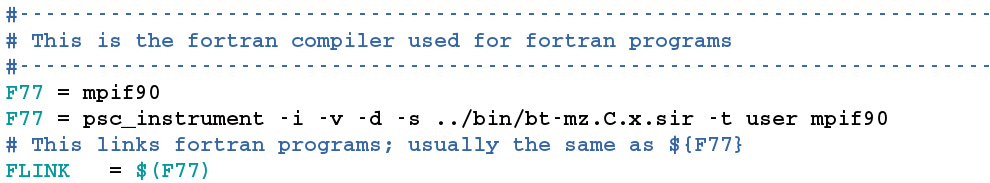
\includegraphics[height=3cm, width=\textwidth]{../BPG/images/uc1_CFS_make_file.png}
	\caption{Change made to make.def file to add {\tt psc\_instrument} wrapper }
	\label{fig:uc1_CFS_make_file}
\end{figure}

In order to test each possible combination of compiler flags, PTF recompiles the application with each combination. PTF is informed about the compilation steps and arguments using the cfs\_config.cfg file, as mentioned in the CFS Plugin User's Guide (available on the PTF website). A template for the configuration file is installed along with the PTF installation. A configuration file used for this example can be seen in Figure \ref{fig:uc1_cfs_config}.

\begin{figure}[H]
	\centering
	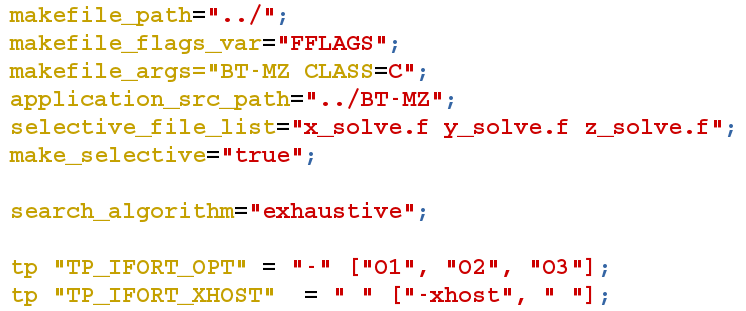
\includegraphics[scale=0.65]{../BPG/images/uc1_cfs_config.png}
	\caption{An example of a configuration file for the CFS plugin.}
	\label{fig:uc1_cfs_config}
\end{figure}


\subsubsection{Running the application with PTF for the first time}
Subsequent to this build step, the BT-MZ application is executed using the PTF {\tt psc\_frontend} command as shown in the PTF User's Guide \cite{PTFguide}. After successful execution, the optimal combination of compiler flags along with a summary of results for each combination is reported by the CFS plugin. For the example that we provide here, the search for the optimal combination of flags took approximately 4697 seconds. This overhead is expected because running PTF for this basic example involves recompilation and re-execution of the application with each combination of the selected compiler flags. Sample output of the PTF execution for the BT-MZ example discussed here is shown in Figure \ref{fig:uc1_cfs_output}.

\begin{figure}[H]
	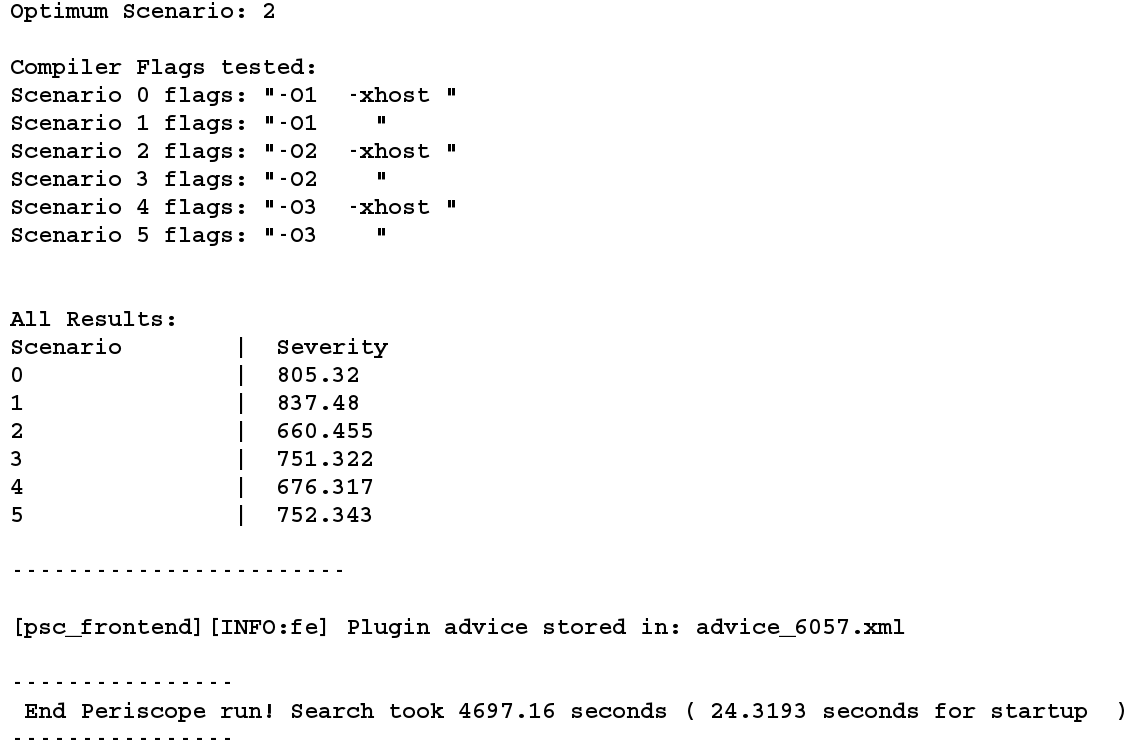
\includegraphics[width=\textwidth]{../BPG/images/uc1_cfs_output.png}
	\caption{Sample output of PTF execution for the BT-MZ benchmark in naive mode.}
	\label{fig:uc1_cfs_output}
\end{figure}

\subsubsection{Reducing the overall execution time using a phase region}

The PTF User's Guide explains the concept of a \emph{phase region}. Many HPC applications have a global progress loop, e.g., going through the simulated time steps. The execution of the loop body for a single time step is called a phase. The phase region, i.e., the loop body, can be marked for PTF in the source code as a \emph{user region}. If the phase region is given, PTF will perform all experiments for a single iteration instead of executing the entire loop and thus, significantly reducing the tuning time. If no phase region is marked via a user region, the main program region is used as the default phase region. 

In our example, BT-MZ has a main time-stepping loop with a trip count of 200, where the same type and amount of computation was executed for each iteration of the loop.  A PTF user region can therefore be placed around the body of this computationally dominant loop. Only two pragma lines are required to be inserted into the BT-MZ source code, representing the start and end of the user region, respectively. For the BT-MZ example, this results in PTF executing only one iteration of the time-stepping loop rather than the full 200 iterations, reducing the execution time of PTF to approximately 227 seconds (relative to 4697 seconds without User Regions). Sample output from a PTF run using the phase region approach is shown in Figure \ref{fig:uc1_user_regions}.

\begin{figure}[H]
	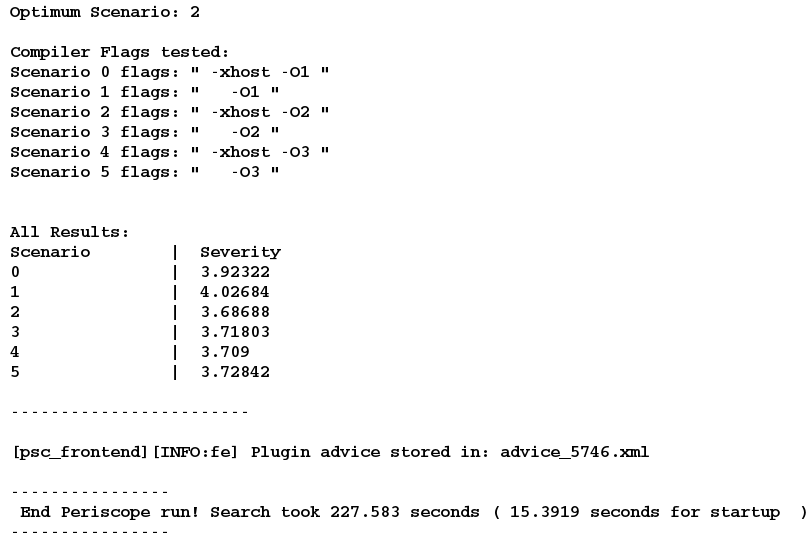
\includegraphics[width=\textwidth]{../BPG/images/uc1_user_regions.png}
	\caption{CFS output for the BT-MZ application with a marked phase region and selective make enabled.}
	\label{fig:uc1_user_regions}
\end{figure}

\subsubsection{Reducing initialization time}
The PTF User's Guide provides information on the ``fast starter'' flag which can reduce the amount of time spent in the initialization of PTF. For example, by passing {\tt --starter=FastInteractive} to the {\tt psc\_frontend} command,  the total execution time for PTF can be reduced further to approximately 161 seconds for the BT-MZ example described here (reducing the time spent in initialization time from approximately 20 seconds to 5 seconds. Sample output showing the effect of {\tt --starter=FastInteractive} can be seen in Figure \ref{fig:uc1_fast_interactive}.

\begin{figure}[H]
	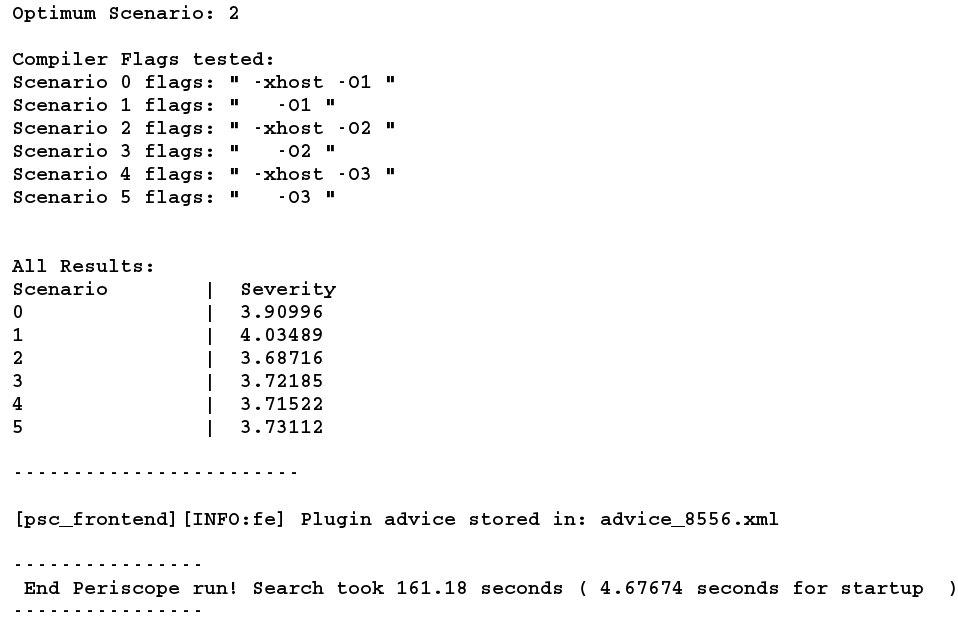
\includegraphics[width=\textwidth]{../BPG/images/uc1_fast_interactive.png}
	\caption{Sample output for the BT-MZ appliation showing the reduction in time spent in initialization of PTF by using the FastInteractive flag.}
	\label{fig:uc1_fast_interactive}
\end{figure}

\subsection{Manual instrumentation}
Manual instrumentation is an important technique to be exploited when dealing with codes that use complex language constructs and that are consequently difficult to instrument using the built-in {\tt psc\_instrument} command (it is often useful for C++ codes). In our second use case we will manually instrument a C++ application and run it using the CFS plugin. The following subsections will walk through each step involved in the manual instrumentation of the code and its significance. We instrument code in order to inform PTF about computationally intensive parts of a given code so as to steer the focus of PTF  tuning efforts. These steps mainly involve identifying the computationally intensive parts of the code through profiling, and then marking them with specific PTF library calls . The build procedure is subsequently updated to link against the PTF libraries to make these functions available. Finally, a {\tt SIR} file is created to convey manual instrumentation information to PTF.

\subsubsection{Application background}
By way of demonstrating best practices on manual instrumentation we will focus on the C++ LULESH (\textbf{L}ivermore \textbf{U}nstructured \textbf{L}agrangian \textbf{E}xplicit \textbf{S}hock \textbf{H}ydrodynamics) \cite{LULESH} code. LULESH is one of the proxy applications proposed by Lawrence Livermore National Lab (LLNL) as part of co-design efforts to address exascale challenges. By its nature, LULESH is a highly simplified application, hard-coded to only solve a simple Sedov blast problem with analytic answers. It represents the numerical algorithms, data motion, and programming style typical in HPC applications written in C or C++.

\subsubsection{Finding the phase region}

To identify the computationally intensive parts of LULESH we will profile the code using gprof by adding the {\tt -pg} compiler flag. This requires updating the Makefile of the application. After executing the newly compiled binary we obtain the profiling data in the form of a binary file named {\tt gmon.out}. Using a tool such {\tt gprof} allows us see the amount of time spent in each function of our application. Figure \ref{fig:uc3_gprof_output} shows partial output from the gprof profile of LULESH running in sequential mode, showing that the majority of time during execution was spent in the {\tt LagrangeLeapFrog} function.
	
\begin{figure}[H]
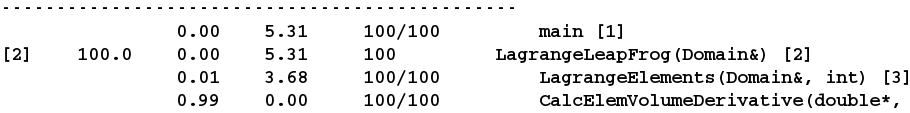
\includegraphics[width=\textwidth]{../BPG/images/uc3_gprof_output.png}
\caption{Partial output from {\tt gprof} showing hotspot functions in LULESH.}
\label{fig:uc3_gprof_output}
\end{figure}
	
Inspecting the source code reveals that the {\tt LagrangeLeapFrog} function is called within an iterative time-stepping loop (a so-called`` phase region"). Figure \ref{fig:uc3_timestep_loop} shows a segment of LULESH source code from the {\tt lulesh.cc} file, containing the while loop which iterates over a given number of time-steps.

\begin{figure}[H]
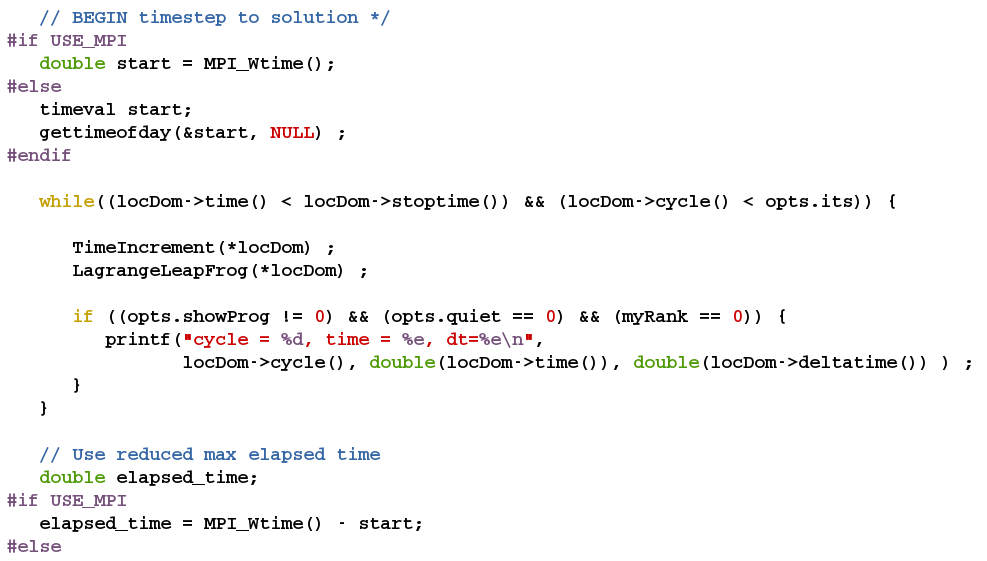
\includegraphics[width=\textwidth]{../BPG/images/uc3_timestep_loop.png}
\caption{The compute intensive while loop interating over the timesteps and calling the {\tt LagrangeLeapFrog} function in LULESH.}
\label{fig:uc3_timestep_loop}
\end{figure}
	
At this stage, we will convey this information about the computationally intensive part of the code to PTF by placing the user region around this segment of the code.
	
\subsubsection{Marking the PTF region in the source code}

To start with the instrumentation we need to mark the beginning and end of the application. Figure \ref{fig:uc3_start_main_region} shows how we mark the beginning of an application using the PTF region, and Figure \ref{fig:uc3_end_main_region} shows the end of PTF region.

The following guidelines need to be followed when marking the start of a PTF region in the example code we work with here (LULESH):
		
\begin{itemize}
	\item Firstly, we have to include a header file {\tt mrimonitor.h}.

	\item Then we need to find the {\tt main} function of the application and declare some of PTF-specific variables.

	\item Next we call the {\tt startMonLib()} function to start a monitoring library.

	\item We then insert a call to the {\tt startRegion()} function with the third argument as the line number where the call to start a monitoring library is made.

	\item Finally, we put the content of the entire {\tt main} function into the code block surrounded by the curly braces.
\end{itemize}
	
	\begin{figure} [H]
		\centering
		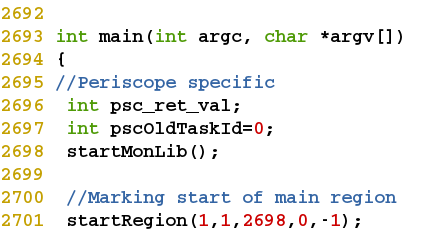
\includegraphics[scale=0.75]{../BPG/images/uc3_start_main_region.png}
		\caption{The {\tt main} function is marked with the start of a PTF region.}
		\label{fig:uc3_start_main_region}

	\end{figure}
	
		The following guidelines need to be followed while marking the end of a PTF region.
		\begin{itemize}
			\item Assign a zero value to {\tt psc\_ret\_val} variable.
			\item Make a call to {\tt endRegion()} function with the same arguments as that of the {\tt startRegion()} function.
			\item Stop the monitoring library by calling {\tt stopMonLib()} function.
			\item Place these calls before the {\tt MPI\_Finalize()} call.
		\end{itemize}

	\begin{figure}[H]
		\centering
		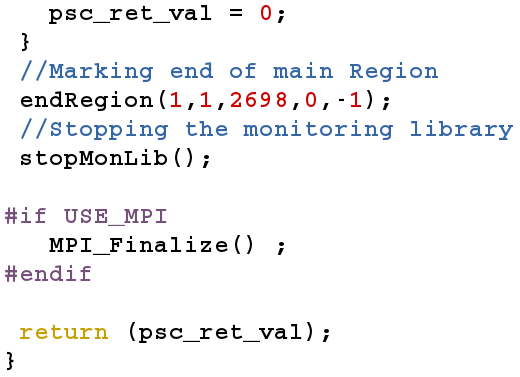
\includegraphics[scale=0.6]{../BPG/images/uc3_end_main_region.png}
		\caption{The end of the PTF region is marked with in the {\tt main} function.}
		\label{fig:uc3_end_main_region}		
	\end{figure}

\subsubsection{Marking a user region in the source code }

A user region can be used to mark the phase region of the application. It then identifies a part of the code where we want PTF to focus it's optimization efforts. User region pragmas are placed around computationally intensive code sections. In the case of a computationally intensive loop traversing a high trip count, performance of a single iteration of the loop for a particular optimization can often be representive of the overall performance of an application for that optimization. When such a loop is marked as a User Region, PTF executes the loop for only a single iteration to measure the performance improvements.
	
	\begin{figure}[H]
		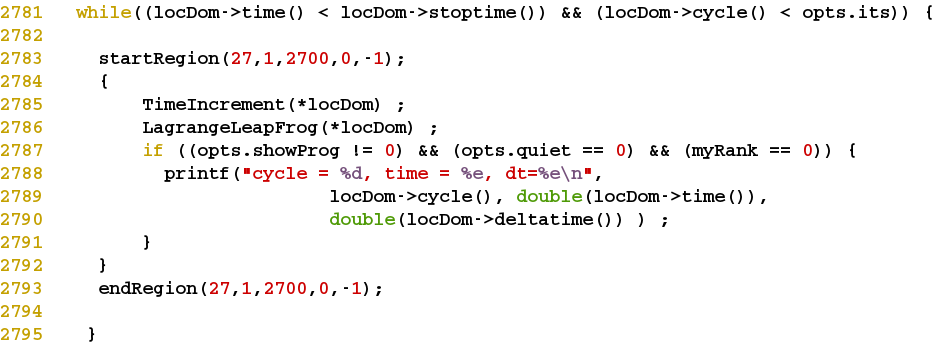
\includegraphics[width=\textwidth]{../BPG/images/uc3_instrumented_loop.png}
		\caption{Instrumented version of the timestep loop.}
		\label{fig:uc3_instrumented_loop}
	\end{figure}

Figure \ref{fig:uc3_instrumented_loop} shows the updated time-stepping loop. The following guidelines need to be followed when marking code with a user region.
	
	\begin{itemize}
		\item Call {\tt startRegion()} and {\tt endRegion()} functions at the beginning and end of the loop. Make a note that both the function calls are inside the loop.
		\item The third parameter in the function is the line number of the statement before the outer {\tt startRegion()} call.
		\item The user region marking the phase region entails a collective synchronization. PTF configures application monitoring in {\tt startRegion()} and {\tt endRegion()}. This configuration leads to a barrier synchronization. 
	\end{itemize}
	
\subsubsection{Updating makefile to link against PTF libraries}

When instrumenting the code we include the {\tt mrimonitor.h} header file and insert function calls {\tt startRegion} and {\tt endRegion()} to mark the region to be instrumented. While compiling this manually instrumented code we need to inform the compiler about the location of the header file to include it, and also inform the linker about the name and location of the libraries containing the necessary function calls.
	
	\begin{figure}[H]
		\centering
		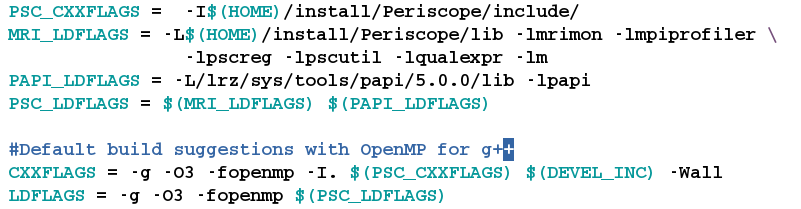
\includegraphics[scale=.65]{../BPG/images/uc3_makefile.png}
		\caption{Updated {\tt Makefile} to find PTF header files and link the PTF libraries.}
		\label{fig:uc3_makefile}
	\end{figure}
	

In Figure \ref{fig:uc3_makefile} we show an updated {\tt Makefile} for LULESH. Relevant changes include -
	
	\begin{itemize}
		\item The path for the PTF headers is provided to compiler by adding to {\tt CXXFLAGS}.
		\item The path and name of the PTF libraries are provided using {\tt LDFLAGS} variable.
		\item Additional libraries  are pointed to by aggregating them into the {\tt PSC\_LDFLAGS} variable.
	\end{itemize}
	
	\subsubsection{Generating a {\tt SIR} File}
	
By way of a {\tt SIR} file we can inform PTF about the outer and User Regions generated during the manual or automatic instrumentation, with an example {\tt SIR} file shown in Figure~\ref{fig:uc3_sir_file} .
	
	\begin{figure}[H]
		\centering
		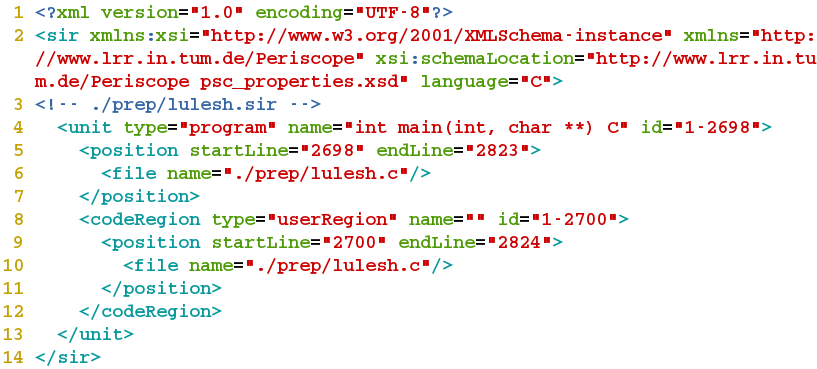
\includegraphics[scale=.65]{../BPG/images/uc3_sir_file.png}
		\caption{{\tt SIR} file}
		\label{fig:uc3_sir_file}
	\end{figure}
	
To generate a {\tt SIR} file one can follow template or any existing {\tt SIR} file and update it using the guidelines below to suit a given application.

\begin{itemize}

\item Update the {\tt id} field of a unit tag, to 1-(line number of a line where the call to {\tt startMonLib()} is made). The id of a region is composed of the two numbers, you can choose both but unique.

\item The {\tt position} tag under the unit tag should contain {\tt startLine} as a line number specified in the outer tag after 1  and {\tt endLine} should be the line where the outer region ends.

\item The {\tt file} tag should contain the value {\tt name} in the {\tt ./\textless file\_name\textgreater.c}.  The name of the file containing the outer region should go here.

\item The {\tt codeRegion} should have {\tt id} as 1-(line number of a line where the call to {\tt startRegion()} is made) and {\tt type} should be {\tt userRegion}.

\item The {\tt position} and {\tt file} tag should follow the same format as the {\tt position} tag used above.
		
		
\end{itemize}	
	
\subsubsection{Executing the instrumented application with PTF}

Once the instrumentation is completed, the execution of the application is carried out in the same way as of an application automatically instrumented with the {\tt psc\_instrument} command. In this case, we use the following commands:

\begin{verbatim}
      module load gcc ace/6.1 papi
      module load boost/1.45 gcc mpi.intel
      
      psc_frontend --apprun="./lulesh2.0" --sir="./lulesh.sir"
                   --mpinumprocs=8 --tune=compilerflags
\end{verbatim}

The \texttt{module load} commands configure an environment on the SuperMUC system with paths for the necessary libraries and the \texttt{psc\_frontend} command is used to start the tuning running the CFS plugin. Here, we have used the same configuration file {\tt cfs\_config.cfg} as that used for the BT-MZ use case.
		
	
\subsubsection{Improving the accuracy of PTF results}
In the case of an instrumented applications with a single iteration of a computationally intensive loop executing for a short amount of time, tuning results may not be consistent. This is mainly due to OS noise or the resolution of the instrumentation. In such cases we can modify the code by increasing the number of iterations to be instrumented in order to obtain consistent results. This can also be achieved by loop splitting. Figure \ref{fig:lulesh_split_loop.png} shows the version of LULESH code shown in Figure\ref{fig:uc3_instrumented_loop} after splitting the loop into two loops. In the new version, a user region is placed around the inner loop which runs for 1000 iterations.

\begin{figure}[H]
	\centering
	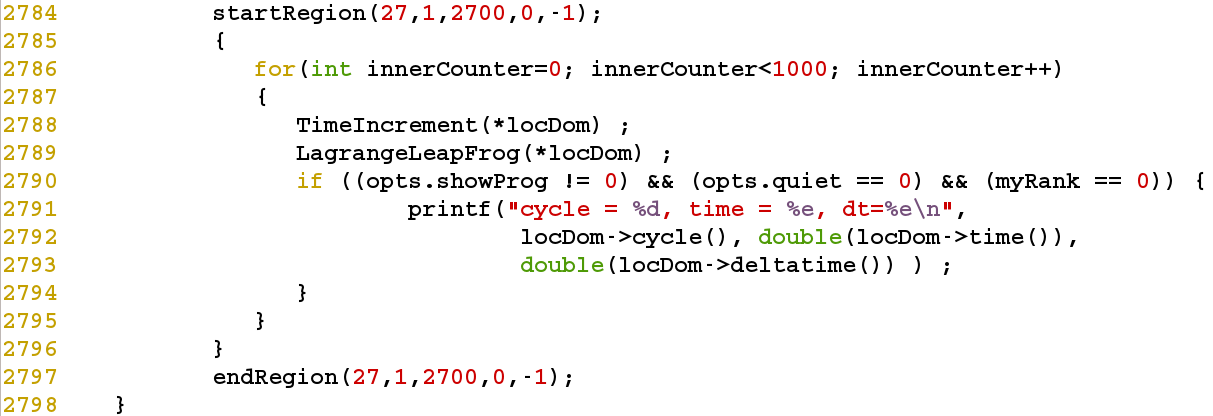
\includegraphics[width=\textwidth]{../BPG/images/lulesh_split_loop.png}
	\caption{Splitting the loop to execute more iterations in the User Region in LULESH.}
	\label{fig:lulesh_split_loop.png}
\end{figure}

\subsubsection{Results for LULESH}
	\begin{itemize}
	\item \textbf{CFS Plugin}

Figure \ref{fig:uc3_cfs_results_exec_time} demonstrates that the combination of the compiler flags suggested by PTF results in ~9.5\% improvement in the overall execution time of LULESH.
	
	\begin{figure}[H]
	\centering
	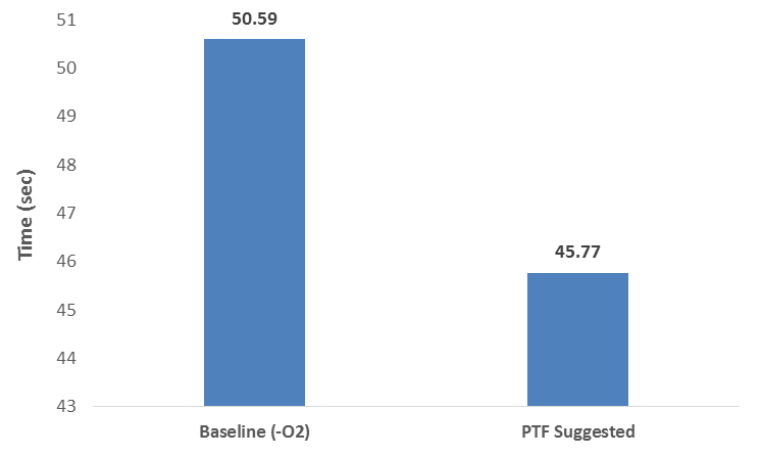
\includegraphics[scale=.60]{../BPG/images/uc3_cfs_results_exec_time.png}
	\caption{Execution time with the optimal compiler flags suggested by PTF and the baseline reading taken without using PTF.}
	\label{fig:uc3_cfs_results_exec_time}
\end{figure}
	\end{itemize}

\subsubsection{Additional tips}
\begin{itemize}

\item It is recommended to add a delay of one or more executions of the phase region in the {\tt psc\_frontend} command using the {\tt --delay} flag to avoid the warm up phase of the application.

\item Check the reproducibility of the measurements.

\end{itemize}

\clearpage

\section{Best Practice on how to use the PTF Tuning Plugins}
\label{sec:chapter4}
In the previous section we focused on walking through two examples of how to best employ PTF on sample applications with the CFS plugin. In this section we provide an overview of the features of each of the PTF plugins which can help to employ PTF and the plugins more effectively as part of a typical PTF tuning workflow.


\subsection{Compiler Flags Selection Plugin}

By way of guiding the user on how to best exploit the CFS plugin, we will focus on two applications from the CESAR suite of exascale proxy applications \cite{CESAR}, NEKBONE and MOCFE. The NEKBONE proxy application is a thermal hydraulics simulation code for  reactor simulations that solves the Poisson equation, Helmholz equation, as well as other differential equations. It is an MPI-based FORTRAN application consisting of 13 files. For the example discussed here, the application was executed with 8 processes and 50 elements per process, a polynomial order of 10, and without the multi-grid preconditioner (i.e. `Example~3' in the provided source code). 

The MOCFE application simulates the main procedures in a 3D method of characteristics (MOC) code for numerical solution of the steady state neutron transport equation.  3D-MOC features heterogeneous geometry capability, high degree of accuracy, and potential for scalability. It is a FORTRAN~90 MPI application consisting of 36 files. We have instrumented the inner loop of {\tt Method\_FGMRES.F90} as a phase\_region of the application. For the example cases described here MOCFE was executed with 16 processes and a Krylov iteration size of 60.


\subsubsection{Using different search algorithms}\label{sec:cfs-search}

The CFS plugin searches for the best possible combination of compiler flags from a list of flags provided in the \texttt{cfs\_config.cfg} file of the plugin. It uses one of five search algorithms, i.e., \textit{Exhaustive Search}, \textit{Random Search}, \textit{Individual Search}, \textit{Genetic Search}, and \textit{Machine Learning-based Random Search} for selecting the best combination of flags. In general, the Individual Search strategy provides good results and is recommended as a good starting point. The Genetic Search and Random Search algorithms can be used in combination with Machine Learning to perform a broader search.

The search algorithms of the CFS plugin are described below:

\begin{itemize}
\item \textit{Exhaustive Search (ES):} The plugin compiles and executes the application with all combinations of the specified compiler flags.
\item \textit{Random Search (RS):} The plugin randomly selects combinations of flags.
\item \textit{Individual (IS):} This algorithm adds-up each compiler flag one after the other from the tuning parameter list in the order used  in the specification file.
\item \textit{Genetic Search (GS): } GS searches for the combination of compiler flags based on the GDE3 genetic algorithm.
\item \textit{Machine learning based Random Search (MLRS): } MLRS uses the Tuning Database of PTF, which is a collection of CFS tuning results for different applications, to model and predict the suitable compiler flags for the current application. The database, in our case, was filled with the NAS parallel benchmark experiments.
\end{itemize}

For the example cases discussed here, we can run all of these algorithms (apart from ES due to the huge number of scenarios) on the NEKBONE application. In the case of the NEKBONE application, the body of the progress loop in the NEKBONE application was marked as a User Region and we also use the following CFS plugin specific features: i) the \textit{Selective Make} option of the CFS plugin to recompile only compute intensive files instead of the entire application and ii) the \textit{Remote Make} option to perform the compilation on the login nodes of SuperMUC, the supercomputer at LRZ that we run our use cases on. For the use-cases described here the compiler flags were pre-defined in the {\tt cfs\_config.cfg} file of the CFS plugin.

We focus on the following FORTRAN compiler flags of Intel's {\tt ifort} compiler when auto-tuning NEKBONE using the CFS plugin:

\begin{verbatim}
tp "TP_IFORT_OPT" = "-" ["O2", "O3", "O4"];
tp "TP_IFORT_XHOST"  = " " ["-xhost", " "];
tp "TP_IFORT_UNROLL" = " " ["-unroll", " "];
tp "TP_IFORT_VERSION" = " " ["-opt-multi-version-aggressive", " "];
tp "TP_IFORT_FMA" = " " ["-fma", " "];
tp "TP_IFORT_INLINE" = " " ["-finline-functions","-fno-inline-functions"];
tp "TP_IFORT_PREFETCH" = "-opt-prefetch=" [1,4,1];
tp "TP_IFORT_UNROLL" = "-unroll" [1,16,4];
tp "TP_IFORT_OPTBLOCK" = "-opt-block-factor=" [1,3,1];
tp "TP_IFORT_STREAM" = " " ["-opt-streaming-stores always",
          "-opt-streaming-stores never", "-opt-streaming-stores auto"];
tp "TP_IFORT_IP" = " " ["-ip", " "];
\end{verbatim}

Figure~\ref{fig:nek_comparisons} compares the execution times for the different search algorithms for the NEKBONE application for a given number of experiments.

\begin{figure}
        \centering
        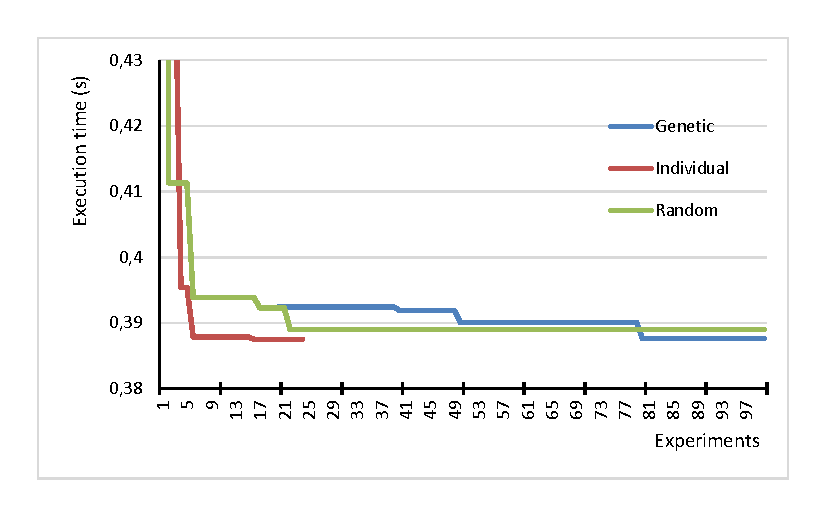
\includegraphics[width=13cm]{../BPG/CFS/CFS-Nekbone-Comparison.pdf}
         \caption{Comparison of IS, GS, and RS for NEKBONE.}
     \label{fig:nek_comparisons}
\end{figure}

It can be seen that all three search algorithms converge to approximately the same execution time for the instrumented application (~0.38 seconds). While the IS algorithm results in the best execution time after only five experiments, the RS algorithm requires 22 experiments and the GS algorithm requires 80 experiments to obtain the shortest execution time for the instrumented application, thus demonstrating the potential advantages of some search algorithms over others when using the CFS plugin. As mentioned, the Individual Search strategy generally provides good results and is recommended as a good starting point when employing the CFS plugin.

\subsubsection{Reducing the compilation time for selected flag combinations} \label{sec:cfs-selective-make}

The \textit {Selective Make} feature of the CFS plugin allows users to reduce the compilation time for a selected combination of flags by recompiling only significant target application files, i.e., files that account for most of the execution time. To demonstrate the impact of this feature here, we apply the CFS plugin (with Individual Search) to the NEKBONE and MOCFE applications . As can be seen from Table~\ref{tab:cfs-recompilation}, the compilation time for the applications differs significantly between recompiling the whole application and recompiling only the significant files using Selective Make. Indeed, for applications composed of many files the Selective Make feature generally leads to a significant reduction in the overhead of searching through CFS parameter spaces and is recommended to CFS plugin users to improve productivity.

\begin{table}
    \centering
    \begin{tabular}{|c | c| c | c | c |}
    \hline
      & \multicolumn{2}{c}{Full Compile} & \multicolumn{2}{|c|}{Selective Compile}\\\hline
     Code & \#Files & Time (s) & \#Files & Time (s)\\
    \hline\hline
    MOCFE	&36 &32.12& 4 &4.503\\[1ex]
    NEKBONE &13 &45.16 &1 &2.22\\[1ex]  \hline
    \end{tabular}
    \caption{Compilation time for the whole application relative to compilation time selecting only the most significant application files.}
\label{tab:cfs-recompilation}
\end{table}

Table~\ref{tab:cfs-selective-influence} compares the results running MOCFE and NEKBONE with the full compilation and the compilation using Selective Make. The results demonstrate that selective compilation leads to a significant reduction of the search time while the results vary only slightly, since the most time consuming routines were recompiled anyway.

\begin{table}
    \centering
    \begin{tabular}{|c | c| c | c | c |}
    \hline
      & \multicolumn{2}{c}{Full Compile} & \multicolumn{2}{|c|}{Selective Compile}\\\hline
     Code & Search (s) & Exec (s) & Search (s) & Exec (s)\\
    \hline\hline
    MOCFE	&1498 &8.4& 855 & 8.3\\[1ex]
    NEKBONE &1950 & 0.37 & 914 & 0.38\\\hline
    \end{tabular}
    \caption{Comparison of search time and resultant execution time for selective compilation.}
\label{tab:cfs-selective-influence}
\end{table}


\subsubsection{Measuring significant routines} \label{para:cfs-significant-routines}

The CFS plugin also allows users to determine the best flag combinations per file. This is based on the identification of routines that take up the majority of computation time in each file selected for selective compilation, where the effect of the compiler flags on the execution of these routines is used to identify the file-specific best flag combination. To demonstrate this feature, we focus on the BT-MZ application as used in section 2 of this guide and run the application with 4 MPI processes and problem size C from the BT-MZ test cases. We use Machine Learning based Random Search with 5 samples. The results presented in Table~\ref{tab:cfs-routine} were achieved for the five samples:


\begin{table}
    \centering
    \begin{tabular}{|l | r| r | r | r |r |}
    \hline
     Scenario & Total & x\_solve & y\_solve & z\_solve & compute\_rhs \\
    \hline\hline
    0	& 4.04 & 1.14 & 1.16 & 1.26 & 0.42\\[1ex]
    1	& 4.03 & 1.13 & 1.15 & 1.25 & 0.42\\[1ex]
    2	& 4.02 & 1.13 & 1.15 & 1.25 & 0.42\\[1ex]
    3	& 3.94 & 1.10 & 1.12 & 1.20 & 0.44\\[1ex]
    4	& 3.93 & 1.10 & 1.13 & 1.19 & 0.44\\[1ex]\hline
    \end{tabular}
    \caption{Tuning results for individual subroutines in NPB BT-MZ.}
\label{tab:cfs-routine}
\end{table}

The following flags were tested in the scenarios:

\begin{enumerate}
  \item {\tt -O3  -xhost        -fma  -fno-inline-functions -opt-prefetch=4 -unroll13 -opt-block-factor=1  -opt-streaming-stores never}
  \item {\tt -O3  -xhost        -fma  -finline-functions -opt-prefetch=4 -unroll13 -opt-block-factor=1  -opt-streaming-stores auto}
  \item {\tt -O3  -xhost        -fma  -finline-functions -opt-prefetch=3 -unroll13 -opt-block-factor=3  -opt-streaming-stores auto}
  \item {\tt -O3  -xhost        -fma  -finline-functions -opt-prefetch=1 -unroll1 -opt-block-factor=3  -opt-streaming-stores always}
  \item {\tt -O3  -xhost        -fma  -fno-inline-functions -opt-prefetch=2 -unroll1 -opt-block-factor=3  -opt-streaming-stores always  -ip}
\end{enumerate}

Subroutines {\tt x\_solve}, {\tt y\_solve}, and {\tt z\_solve} are very similar and the best configurations were found to be scenario~4 for {\tt x\_solve} and {\tt z\_solve}. A very small time difference was reported for scenarios 3 and 4 for {\tt y\_solve}. These scenarios are almost identical and thus we can summarize that all three routines work well with scenario~4. For subroutine {\tt compute\_rhs} a more significant difference can be seen for scenarios 0-2 and 3-4. Therefore, the plugin recommends to compile file {\tt rhs.f} with the flag combination from scenario~1. The global optimum is scenario~4 since the all three {\tt solve} routines are almost three times as time consuming as {\tt compute\_rhs}.

\subsubsection{Remote Make}
Finally, compute nodes of HPC systems often have a light-weight version of Linux and may not have all the necessary files to recompile the application. In order to recompile the application with the different flags combinations, the CFS plugin supports remote building of the application. The compilation is then run on, for example, a login node via \texttt{ssh}. Please consult the CFS Plugin User's Guide on how to configure the CFS plugin to use \texttt{remote make}.




\clearpage

\subsection{Parallel Patterns Plugin}

By way of guiding the user on how to best exploit the Parallel Patterns plugin, we will focus on the FaceDetect application \cite{FaceDetect}. The FaceDetect application uses an image-processing pipeline built on top of the PEPPHER framework. Within PEPPHER, pipeline patterns are expressed using annotated while-loops that comprise calls to multi-architectural components. The high-level FaceDetect code is shown in Figure \ref{fig:facedetect}. The application uses a four stage pipeline to perform detection of human faces on a stream of images. 

\definecolor{gray}{rgb}{0.9,0.9,0.9}
\definecolor{darkgreen}{rgb}{0.0,0.6,0.0}
\definecolor{codegreen}{RGB}{0,116,0}
\definecolor{codebrown}{RGB}{100,56,32}
\definecolor{codebackgroundcolor}{rgb}{0.933,0.925,0.882}
\definecolor{xmlelement}{RGB}{187,68,165}
\definecolor{xmlattr}{RGB}{0,0,0} %{167,125,58}
\definecolor{xmlval}{RGB}{207,49,37}
\lstset{
	frame=tb, 
    basicstyle=\scriptsize \ttfamily, 
    numberstyle=\footnotesize,
    showstringspaces=false,
    captionpos=b,
    breaklines=true, 
    language=c++,
    tabsize=2,
    xleftmargin=2em, framexleftmargin=2em, framextopmargin=0.5em, framexbottommargin=0.5em,  aboveskip=1.5em, belowskip=0.1em,  rulesepcolor=\color{gray}, abovecaptionskip=.5\baselineskip, belowcaptionskip=.1\baselineskip, backgroundcolor=\color{codebackgroundcolor}, escapechar=^
    }
    
The Parallel Patterns plugin for PTF supports automatic performance tuning of  high-level pipeline patterns built on top of the PEPPHER framework. The plugin searches for the best combination of pattern-specific parameters, parameters exposed by the runtime system, and machine-specific parameters such that execution is optimized for a given workload and target architecture.

The plugin for Parallel Patterns allows for the restriction of a potentially large search space via: 

  \begin{itemize}
    \item tuning range specifications for stage replication factors and stage buffer sizes by means of source code directives
    \item tuning range specifications for all tuning parameters via configuration file 
    \item performance analysis to focus tuning on the most time-consuming stage
  \end{itemize}

\begin{figure}[h]
\centering
\begin{lstlisting}
#pragma pph pipeline
while ( inputstream >> file ) {
    ReadImage ( file , image );
    ^\color{codebrown}{\#pragma pph stage replicate(?) buffer(?)}^
    ResizeAndColorConvert ( image, oimage );
    ^\color{codebrown}{\#pragma pph stage replicate(?) buffer(?)}^
    DetectFaces( oimage );
    WriteFaceDetectedImage ( file , oimage );
}
\end{lstlisting}
\caption{A pipeline pattern for face detection in a stream of images. The "?" symbols within the annotations indicate that the tuning ranges for \texttt{ResizeAndColorConvert} and \texttt{DetectFaces} stages should be automatically determined.}
\label{fig:facedetect}
\end{figure}

\subsubsection{Default behavior}

The total number of tuning scenarios in the search space is created as a crossproduct of the value ranges of all available tuning parameters. By default, for each of the tuning parameters the tuning range of possible values is determined by the system as follows:  

\begin{itemize}
\item for each stage replication factor that has been annotated with the "?" in the high-level code, the range of the stage replication factor is set to [1:(\textit{max\_execution\_units - number\_of\_pipeline\_stages - 1}):1]
\item for each buffer size, that has been annotated with the "?" in the high-level code, the range of the buffer size is set to [\textit{max\_execution\_units}:\textit{max\_execution\_units}*3:\textit{max\_execution\_units}]
\item the NCPUS range is set to [1:\textit{max\_cpu\_cores}:1]
\item the NGPUS range is set to [0:\textit{max\_gpus}:1]
\item {the SCHEDULING\_POLICY is set to two scheduling policies EAGER and HEFT\footnotemark}
\end{itemize}

These default values are based on the runtime system requirements and on the application testing experience. To minimize oversubscription, the total number of stages plus stage replicas is set to not exceed the number of execution units on the system. The buffer size influences the memory footprint of the application. For each stage, the buffer size is set to have minimum equal to the replication factor of that stage, and to have maximum of that value multiplied by 3.    

\footnotetext{HEFT (Heterogeneous Earliest Finish Time) considers inter-component data dependencies and schedules components to workers taking into account the current system load, available component implementation variants, and historical execution profiles, with the goal of minimizing overall execution time by favoring implementations variants with the lowest expected execution time. EAGER is a simply greedy scheduler. }

Tuning the pipeline on the system with many execution units may require an exploration of a huge search space. For instance, on the system with 16 CPU cores, and 4 GPUs, a full exhaustive search for the FaceDetect application would require an evaluation of 17*3*17*3*16*5*2 = 416,160 scenarios. In Table \ref{tab:fdfullspace} we summarize the possible values for each tuning parameter in this setup. 

\begin{table}[!h]
\begin{center}
\begin{tabular}{ @{} l @{} c }
\hline
\multicolumn{1}{c}{\textbf{ Tuning parameter }} & \textbf{ Possible values } \\
\hline
\hline
{ \texttt{ResizeAndColorConvert} Replication Factor}  & {1, 2, 3,.., 17} \\ \hline 
{ \texttt{ResizeAndColorConvert} Buffer Size} & {20, 40, 60}  \\ \hline  
{ \texttt{DetectFaces} Replication Factor}  &  {1, 2, 3,.., 17} \\ \hline 
{ \texttt{DetectFaces} Buffer Size} & {20, 40, 60} \\ \hline   
{ Number of CPU cores} & {1, 2, 3,.., 16} \\ \hline 
{ Number of GPUs} & {0, 1, 2, 3, 4} \\ \hline 
{ Scheduling Policy} & {``EAGER'', ``HEFT''}  \\ \hline 
\end{tabular}
\vspace{4pt}
\caption{Tuning parameters and their values on the PHIA system for the setup with no restrictions. }
\label{tab:fdfullspace}
\end{center}
\end{table}

The following three subsections demonstrate how to efficiently restrict the search space, and yet test majority of the performance-relevant scenarios. 
  
\subsubsection{Tuning range specification via directives}
The tuning range source code directives allow users to steer the tuning process of the plugin by specifying values for the stage replication factors and buffer sizes. 
Careful specification of the tuning ranges for such parameters in the high-level code may reduce the total number of scenarios that need to be tested.

For the FaceDetect application tuning, we used these directives to provide tuning ranges for the replication factors of the two middle stages in the pipeline. As shown in Figure \ref{fig:tuningrange}, the user specified tuning range starts with the minimum value of 1, which is incremented by 4 until it reaches the maximum value of 17, resulting in a total of 5 values for each tuning parameter. The minimum value of 1 will reveal if incrementing the replication factor for the certain stage has any effect on the performance. For the maximum value, it is usually good to keep the default of \textit{max\_execution\_units - number\_of\_pipeline\_stages - 1}. This will ensure that oversubscription is avoided. Finally, a good guideline for the increment is actual number of GPUs in the system, since the runtime system needs one CPU core for each GPU card it uses.   
 
\begin{figure}[htb]
\centering
\begin{lstlisting}
#pragma pph pipeline
while ( inputstream >> file ) {
    ReadImage ( file , image );
    ^\color{codebrown}{\#pragma pph stage replicate(1:17:4)}^
    ResizeAndColorConvert ( image, oimage );
    ^\color{codebrown}{\#pragma pph stage replicate(1:17:4)}^
    DetectFaces( oimage );
    WriteFaceDetectedImage ( file , oimage );
}
\end{lstlisting}
\caption{User-provided tuning hints. For the middle stages the tuning ranges for the stage replication factor is specified in  the form {\tt (min:max:step)}.}
\label{fig:tuningrange}
\end{figure}

By specifying tuning ranges for stage replication factors as shown in Figure \ref{fig:tuningrange}, the search space is reduced from 416,160 to 36,000 scenarios.

\subsubsection{Tuning range specification via configuration file}
Another option for enabling users to restrict the search space is by specifying tuning ranges in the SIR file for some or all tuning parameters (including NCPUS, NGPUS). 
In the configuration file, it is a good idea to provide tuning ranges for machine-specific tuning parameters, i.e., NCPUS and NGPUS. For instance, NCPUS parameter may be restricted in a way that the minimum number of CPU cores to be used for execution is equal to the number of pipeline stages, and the maximum is equal to the number of available CPU cores with an increment of 4 (see Figure \ref{fig:sirtuningrange}). As a consequence only 4 values for the NCPUS tuning parameter are considered, further restricting the search space to 9,000 scenarios. The tuning parameters and corresponding values that describe this restricted search space are summarized in Table \ref{tab:fdspaceretricted}.   

\begin{figure}[htb]
\centering
\begin{lstlisting}
...
  ^\color{xmlelement}{<selector}^ ^\color{xmlattr}{tuningActionType}^=^\color{xmlval}{"VAR"}^ ^\color{xmlattr}{tuningActionName}^=^\color{xmlval}{"NCPUS"}^ ^\color{xmlattr}{min}^=^\color{xmlval}{"4"}^ ^\color{xmlattr}{max}^=^\color{xmlval}{"16"}^ ^\color{xmlattr}{step}^=^\color{xmlval}{"4"}^^\color{xmlelement}{/>}^
...
 \end{lstlisting}
 \caption{In order to influence the tuning process\, the SIR file may be altered manually by changing the corresponding \textit{min}\, \textit{max} and \textit{step} values for the desired tuning parameter.}
 \label{fig:sirtuningrange}
\end{figure}

\begin{table}[!h]
\begin{center}
\begin{tabular}{ @{} l @{} c }
\hline
\multicolumn{1}{c}{\textbf{ Tuning parameter }} & \textbf{ Possible values } \\
\hline
\hline
{ \texttt{ResizeAndColorConvert} Replication Factor}  & {1, 5, 9, 13, 17} \\ \hline 
{ \texttt{ResizeAndColorConvert} Buffer Size} & {20, 40, 60}  \\ \hline  
{ \texttt{DetectFaces} Replication Factor}  & {1, 5, 9, 13, 17} \\ \hline 
{ \texttt{DetectFaces} Buffer Size} & {20, 40, 60}  \\ \hline   
{ Number of CPU cores} & {4, 8, 12, 16} \\ \hline 
{ Number of GPUs} & {0, 1, 2, 3, 4} \\ \hline 
{ Scheduling Policy} & {``EAGER'', ``HEFT''}  \\ \hline 
\end{tabular}
\vspace{4pt}
\caption{Tuning parameters and restricted values on the PHIA system.}
\label{tab:fdspaceretricted}
\end{center}
\end{table}

\subsubsection{Focused tuning via performance analysis}
Focused tuning of pipeline patterns via PTF pre-analysis may be enabled via \texttt{--vpattern-focused} command-line switch. In this mode, the plugin uses PTF's pre-analysis to detect the most performance-demanding stage in the pipeline. Once it has been detected, the tuning efforts are focused on the stage replication factor and buffer size of that stage. 

The focused tuning can be used without any additional user-provided hints. In the standalone mode it reduces the search space from initial 416,160 to 8,100. A combination of focused tuning with user-provided tuning ranges may be used to further decrease the search space. 
For the FaceDetect application the stage replication factor for the most performance-demanding stage (\texttt{DetectFaces}), is automatically set to [1:17:1], while for all other stages tuning of stage replication factors (and buffer sizes) is omitted.
As a result, the resulting scenario pool contains only 600 scenarios, significantly reduced from the initial total of 416,160 scenarios.  


Figure \ref{fig:bpg_comp} shows the effect of the different plugin features on the size of the search space. The first blue bar shows the number of scenarios when source code directives were used to restrict the search space from 416,160 to 36,000. The second blue bar represents additional restriction of the search space by adjusting tuning ranges directly in the configuration file. The third blue bar shows the number scenarios when only focused tuning via pre-analysis was used. Finally, the fourth blue bar shows the number of the scenarios when all features were used. 

\begin{figure}[h]
\centering
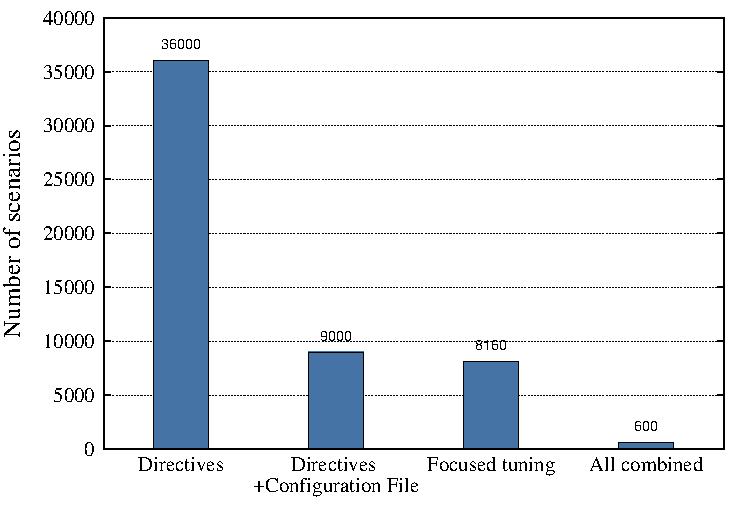
\includegraphics[width=14cm]{../BPG/phia-bpg.pdf}
\caption{Restricting the search space for the FaceDetect application using different plugin features of the Parallel Patterns plugin. }
\label{fig:bpg_comp}
\end{figure}

\subsubsection{Additional tips}
\begin{itemize} 
\item Stage Replication Factors

Stage replication factors determine the number of stage instances executed in parallel and therefore influence the degree of potential parallelism during application execution. Each stage replica will execute in an additional thread. To avoid oversubscription, the total number of stages plus stage replicas should not exceed the number of execution units on the system. On the other hand, if the replication factors are too low, the performance might be limited, so a good guideline is to increase stage replication factors for the stages that have higher performance demands. 
\item Machine-specific Parameters

The machine-specific parameters (NCPUS and NGPUS) are closely related to stage replication factors. The effective usage of system execution units may be hindered if the stage replication factors are not sufficiently high. On the other hand, if the total number of available execution units is small, the replication factor will have no effect. 

\end{itemize}


%\subsubsection{Plugin Features}

%The plugin for Parallel Patterns allows for the restriction of a potentially large search space 
%via:
%   \begin{itemize}
%    \item Tuning range specifications for stage replication factors and stage buffer sizes by means of source code directives: The tuning range source code directives allow users to steer the tuning process of the plugin by specifying values for the stage replication factors and buffer sizes. 
    %As shown in Figure \ref{fig:tuningrange}, the user specified tuning range starts with the minimum value of 1, which is incremented by 4 until it reaches the maximum value of 17, resulting in a total of 5 values for each tuning parameter. 
    
%    \item Tuning range specifications for all tuning parameters via configuration file: Restriction of the search space by specifying tuning ranges in the SIR file for some or all tuning parameters (including NCPUS, NGPUS).
    
%    \item Performance analysis to focus tuning on the most time-consuming stage: In this mode, the plugin uses PTF's pre-analysis to detect the most performance-demanding stage in the pipeline. Once it has been detected, the tuning efforts are focused on the stage replication factor and buffer size of that stage. 
   
%   \end{itemize}


%\subsubsection{Plugin Features}
%\begin{itemize}
%	\item Short description about the available tuning parameters
	
%The pipeline-specific tuning parameters target pipeline structural tuning parameters such as stage replication factors, and sizes of input/output buffers. Machine-specific parameters NCPUS and NGPUS are used to describe available hardware resources such as the number of available CPU cores (or available hardware threads) and number of usable graphic cards. Finally, the runtime-specific parameters include the scheduling policy used by the StarPU runtime system e.g., EAGER (simple greedy scheduler), HEFT (Heterogeneous earliest Finish Time), or similar.  

%The plugin supports follow tuning parameters: 
 %  \begin{itemize}
%	\item \emph{stage replication factor} - the number of stage instances that may be executed in parallel
%	\item \emph{sizes of buffers} - size of I/O buffers that hold data packets passed between pipeline stages
%	\item \emph{number of CPU cores} - number of available CPU cores to be used by the runtime system 
%	\item \emph{number of GPUs} - number of available graphic cards to be used for execution
%	\item \emph{scheduling strategy} - a scheduling policy used by StarPU runtime for scheduling component calls to available execution units of the target system
%   \end{itemize}

%The total number of tuning scenarios in the search space is created as a crossproduct of the value ranges of all available tuning parameters. 
%	\item Search Strategy
	
	
%	 The plugin for Parallel Patterns allows for the restriction of a potentially large search space via: 
	
%	\begin{itemize}	
%		\item If any other search strategy than exhaustive available.
%	\end{itemize}
	
%	\begin{itemize}
%		\item How to decide good replication factor or optimal resource count.
%		\item Selection of parameters to get optimal scenario quickly without exploding search space.
%	\end{itemize}
	
%	\item Use of SIR file to change the parameters
%	\begin{itemize}
%		\item Give range of values for a particular parameters
%	\end{itemize}

%	\item Choice of replication factor and its relation to the number of available resources
%	\begin{itemize}
%		\item Selecting higher replication factor than the resources for I/O, network abound tasks
%		\item How tuning parameters are used by the plugin and role of StarPU runtime. e.g. StarPU might decide to schedule tasks on CPU/GPU or both for some time even when replication factor is one.
%	\end{itemize}



%	\item Scheduling policy
%	\begin{itemize}
%		\item How to select appropriate scheduling policy.
%		\item HEFT uses historical data, how it improves over a period of time, how many runs it requires to see impact on execution time.
%	\end{itemize}
%	\item Buffer size
%	\begin{itemize}
%		\item In which cases buffer size plays important role
%		\item how to anticipate optimal buffer size
%	\end{itemize}
%\end{itemize}

\clearpage


\subsection{Dynamic Voltage Frequency Scaling (DVFS) Plugin}
As an example of how to best employ the features of the DVFS plugin we have chosen the SeisSol application \cite{SeisSol} as our use case here. The SeisSol application is developed by the Department of Earth and Environmental Sciences at the Ludwig-Maximilian University. It is a MPI application written in Fortran 90. The application is used for simulating realistic earthquake scenarios, accounting for a variety of geophysical processes that affect the propagation of seismic waves, e.g. viscoelastic attenuation, strong material heterogeneities and anisotropy. SeisSol contains a computation kernel which simulates the specified number of time steps.

\subsubsection{Extending the search space}

The objective of the DVFS plugin is to tune the energy consumption of an application. The DVFS plugin can be configured with the number of frequencies that the plugin should use for the search space. The models predict one frequency according to the tuning objective. The number of neighboring frequencies (neighbors of the predicted frequencies) to be analyzed can be set. Environment variable PSC\_FREQ\_NEIGHBORS is used for this purpose. The value of this variable specifies the number of neighbors to the right and to the left of the predicted frequency. The maximum value for this variable is limited to 7 neighbors. If the value exceeds 7 neighbors or if it is negative then the plugin will use the default value of 1 neighbor on each side. The user is advised to use a higher number of neighbors when the execution time does not play a role, i.e., when the tuning is completed in an acceptable time-frame for the user. If it is suspected that the model delivers inaccurate predictions, a higher number of frequencies can help mitigate this problem.

Figure \ref{fig:seissol_dvfs_3_nebr} shows the sample output of the DVFS plugin for the SeisSol application with PSC\_FREQ\_NEIGHBORS=3. The tuning objective was to minimize the Energy Delay Product (EDP). 

\begin{figure}[H]
  \centering
  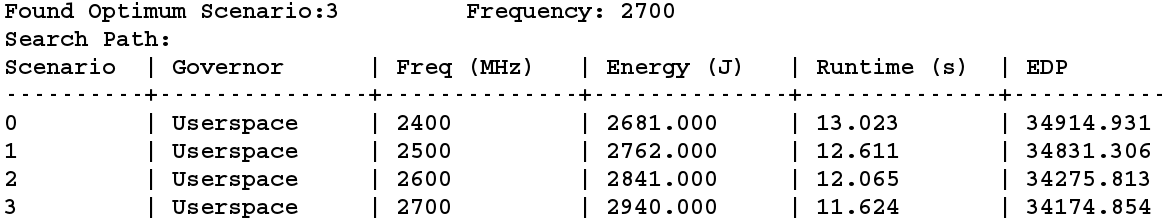
\includegraphics[scale=0.6, width=\textwidth]{../BPG/images/seissol_dvfs_3_nebr.png}
  \caption{Output of the DVFS plugin for inspecting the predicted and three neighbor frequencies.}
  \label{fig:seissol_dvfs_3_nebr}
\end{figure}

The output shows that the three neighbors below the predicted CPU frequency of 2.7\,GHz are measured compared to the default of one neighbor as shown in Figure\ref{fig:uc3_dvfs_model_3_results}. Since 2.7GHz is the highest CPU frequency supported by the Sandy Bridge processors of SuperMUC, only the three lower neighboring frequencies are evaluated. 

\subsubsection{Selection of phase regions}

There are several methods to prepare the application selected for energy tuning. Many scientific codes have a time stepping loop, also known as a phase region. The most common method is to target the phase region in a code for tuning. The phase region is typically the region that consumes the most amount of time. Instrumenting the phase region consists of simply inserting the appropriate directives as follows:

\begin{itemize}
		\item Fortran: \\
		DO i = 1, 10 \\
		!\$ MON USER REGION \\
		kernel... \\
		!\$ MON END USER REGION \\
		ENDDO !Instrumented var \\
		\item C/C++ \\
		for(int i = 0; i \textless 10; i++) \\
		\{ \\
		\#pragma start\_user\_region \\
		kernel... \\
		\#pragma end\_user\_region \\
		\} \\		
\end{itemize}

Not every application has an outermost iterative loop with a time stepping scheme that can be used as a phase region. Either the main region can be used as phase region, resulting in an automatic restart of the application for each experiment, or some other region can be marked a phase region to restrict the tuning to this region. 

PTF user region can also be used to mark code regions also for other purposes then as a phase region. If a single user region is given, this is assumed to be used as phase region in PTF. If multiple user regions are given, the phase region can be identified by an input argument to the PTF frontend. The argument has the format {\tt--phase=``\textless file id \textgreater:\textless region first line \textgreater ''}. For example: 

\begin{verbatim}
    psc\_frontend --apprun="./Seissolxx PAR.par" --mpinumprocs=32 
                  --tune=dvfs --phase="31:809" --sir=SeisSol.sir
\end{verbatim}


If there is no phase region use the command as you would normally do.

Note that there can only be one phase region within the source code and it should be the outer most loop of all other instrumented regions. The presence of phase regions ensure faster automatic tuning, as each experiment is carried out by running one iteration (as opposed to running the entire application per experiment).  It is important not to have significant variations of time among iterations, otherwise the comparisons between experiments will produce wrong results. If the iterations at the phase region are suspected to have variations among them, then do not use a phase region. The loop of the phase region should have at least $2m+1$ iterations, where $m$ is the number of frequencies chosen. One iteration is for the pre-analysis, and $2m$ other iterations for the experiments.

\subsubsection{Multiple tuning objectives}

There are three models used in this plugin to predict the best frequency for a given objective, i.e., one for each of the quantities  \textit{Time}, \textit{Power}, and \textit{Energy}. The rest of the models are derived from these three main models and are used for the tuning objectives. Energy is modeled directly and this is the default model of the DVFS Plugin. Nevertheless, there is an energy model derived from the product of modeled power and time separately (export the environment variable ``export PSC\_DVFS\_MODEL=2'' before running). Variations are not significant between these two energy models and the user is encouraged to use any of the two when tuning for energy consumption.

There are several tuning objectives that can be chosen. You can optimize the energy consumption, the energy delay product, tune for power capping, optimize the total cost of ownership, or tune the energy consumption for an allowed performance degradation. The choice of the metric depends on the needs of the user. Here are some examples:

\begin{itemize}

\item  Consider optimizing the energy consumption when other costs related to time are minimal compared to energy costs. (PSC\_DVFS\_MODEL is either 1 or 2)

\item The energy delay product provides a strong emphasis on time (export PSC\_DVFS\_MODEL=3). The formula has time squared times power.

\item Consider using the total cost of ownership when you need to balance the influence of power-related costs and time-related costs (export PSC\_DVFS\_MODEL=4).

The Total Cost of Ownership (TCO) was used with the following cost formula (given per compute node):

\begin{equation}\label{eq: TCO}
		  TCO = a \cdot P \cdot t + b \cdot t,
\end{equation}

where $P$ is the average power in watts, $t$ the time in seconds, $a$ the cost of the energy  (in the plugin $ a = 2.7 \cdot 10^{-4} [EUR/J]$), $b$ the cost of personnel and other fixed costs amortized over the lifespan of the HPC system (in the plugin $ b = 0.1115 [EUR/s] $).

\item Power capping is used to limit the power and avoid trespassing a system-wide power limit which can generate more costs as electric companies penalize strong oscillations (export PSC\_DVFS\_MODEL=5). The power capping tuning objective uses a maximum power limit of 110 W per node.\\

\item Use PSC\_DVFS\_MODEL=6 when the increase of performance should be greater than an increase in energy  consumption in order to choose higher frequencies and power capping is not needed.

\item Use PSC\_DVFS\_MODEL=7 when the increase of performance should be greater than the increase in power. This case is more restrictive than the previous policy (selected using PSC\_DVFS\_MODEL=6) as it considers power instead of energy.

\item Use PSC\_DVFS\_MODEL=8 when power capping considerations are important. The frequency used will be chosen such that the power used is below the power threshold or have significant performance increase with respect to the nominal frequency 2.0\,GHz.

\item Use PSC\_DVFS\_MODEL=9 when the performance degradation with respect to the nominal frequency should be no more than 10\%.

\end{itemize}
	
Figure \ref{fig:uc2_dvfs_result} shows the execution of the SeisSol application using a default energy model PSC\_DVFS\_MODEL=1 and thus tuning for minimum energy usage. 
	
\begin{figure}[H]
	\centering
	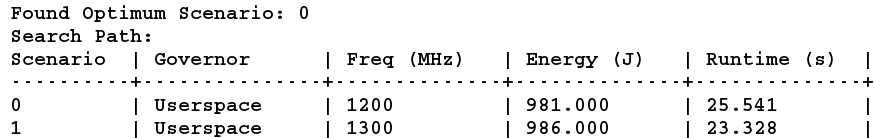
\includegraphics[scale=0.65]{../BPG/images/uc2_dvfs_result.png}
	\caption{Output of the DVFS plugin for energy tuning for SeisSol.}
	\label{fig:uc2_dvfs_result}
\end{figure}

The results show that executing SeisSol at 1.2 GHz would minimize the energy consumed during the execution. When choosing the Energy Delay Product as tuning objective instead of consumed energy, the plugin determines 2.6 GHz as the optimal frequency (Figure \ref{fig:uc3_dvfs_model_3_results}).

\begin{figure}[H]
	\centering
	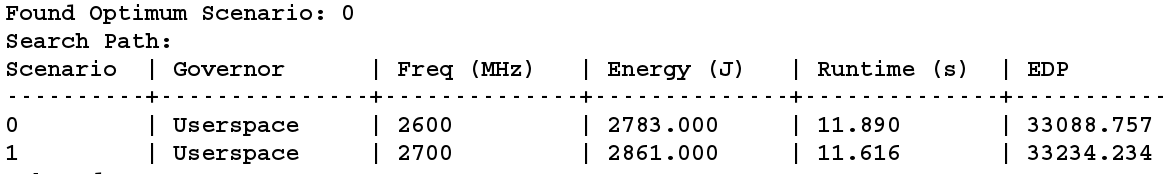
\includegraphics[scale=0.65, width=\textwidth]{../BPG/images/uc3_dvfs_model_3_results.png}
	\caption{Output of the DVFS plugin for tuning the Energy Delay Product for SeisSol.}
	\label{fig:uc3_dvfs_model_3_results}
\end{figure}


\subsubsection{Multiple application regions}

The DVFS plugin can not only determine a global best frequency but also individual best frequencies for different regions of the application. These regions have to be suited for energy tuning, i.e., they have to be coarse enough to amortize for the overhead of changing the processor frequency. 

To demonstrate this feature, three regions were marked in SeisSol for energy tuning. Table~\ref{table:regions}. The two inner regions group similar computations and are included in the phase region (region in calc\_seissol.f90). (In the table each region is given an identification number.)

\begin{table}[htpbH]
\centering
\begin{tabular}{|l|l|l|}
\hline
File & Region First Line & Region ID\\\hline
calc\_seissol.f90 & 489 & 1\\
galerkin3d\_tetra.f90 & 193 & 2 \\
galerkin3d\_tetra.f90 & 289 & 3\\\hline
\end{tabular}
	\caption{Instrumented regions in SeisSol.}
	\label{table:regions}
\end{table}

Tables~\ref{table:calcseis},~\ref{table:galerking3d1}, and~\ref{table:galerking3d2} show the results of for the SeisSol application when run with the tuning objective that optimizes
for energy consumption. Regardless of the tuning objective, the output of the plugin always displays the energy consumption, the runtime, Energy Delay Product ($EDP$), Energy Delay squared Product ($ED^2P$), the average power, and Total Cost of Ownership (TCO). Time and energy (and indirectly average power) are measured and reported on in the output.

\begin{table}[htpbH]
\centering
\begin{tabular}{|c |c |c |c |c |c |c|}
\hline
Frequency & Energy & Runtime & EDP           & EDDP            & Average Power & TCO \\
~[GHz]  & [$J$]  & [$s$]   &  [$J\cdot s$] & [$J\cdot s^2$]  & [Watt]        & [Euro] \\
\hline\hline
1.6       & 1132   & 18.196  & 20597.4    & 374782.4  & 62.2       & 2.3341\\
1.7       & 1143   & 17.075  & 19516.6    & 333244.2  & 66.9       & 2.2121\\
1.8       & 1172   & 16.230  & 19021.3    & 308712.3  & 72.2       & 2.1257\\
\hline
\end{tabular}
	\caption{Energy figures for Region~1.}
	\label{table:calcseis}
\end{table}

\begin{table}[htpbH]
\centering
\begin{tabular}{|c |c |c |c |c |c |c|}
\hline
Frequency & Energy & Runtime & EDP          & EDDP      & Average Power & TCO \\
~[GHz]  & [J]  & [s]   & [J$\cdot$ s] & [$Js^2$]  & [Watt]        & [Euro] \\
\hline\hline
1.6       & 185   & 1.545  & 285.8    & 441.6  & 119.7       & 0.2222\\
1.7       & 185   & 1.548  & 286.4    & 443.5  & 119.5       & 0.2226\\
1.8       & 186   & 1.547  & 287.8    & 445.4  & 120.2       & 0.2227\\
\hline
\end{tabular}
	\caption{Energy figures for Region~2.}
	\label{table:galerking3d1}
\end{table}

\begin{table}[H]
\centering
\begin{tabular}{|c |c |c |c |c |c |c|}
\hline
Frequency & Energy & Runtime & EDP          & EDDP      & Average Power & TCO \\
~[GHz]  & [J]  & [s]   & [J$\cdot$ s] & [$Js^2$]  & [Watt]        & [Euro] \\
\hline\hline
1.6       & 912   & 16.2  & 14805.2  & 240345.1 & 56.2       & 2.0560\\
1.7       & 928   & 15.3  & 14152.7  & 215837.8 & 60.8       & 1.9507\\
1.8       & 971   & 14.6  & 14136.7  & 205814.7 & 66.7       & 1.8852\\
\hline
\end{tabular}
	\caption{Energy figures for Region~3.}
	\label{table:galerking3d2}
\end{table}

These results show that using 1.6\,GHz optimizes the energy consumption of SeisSol for all three regions. The energy savings per region with respect to the worst case scenario are shown in Table~\ref{table:regionsavings}.

\begin{table}[H]
 \centering
 \begin{tabular}{| c | c | }
  \hline
  Region ID & Energy Savings \\\hline\hline
      1     &  3.4\%         \\\hline
      2     &  0.5\%    \\\hline
      3     &  6.1\%	\\
  \hline
 \end{tabular}
 \caption{Energy savings per region.}
 \label{table:regionsavings}
\end{table}

The plugin can be configured to use a tuning objective of either EDP, power capping, or TCO.  The EDP search space is the same as the one shown in Tables~\ref{table:calcseis}, \ref{table:galerking3d1}, and~\ref{table:galerking3d2}. The results for the case of EDP point to an optimization when using 1.8\,GHz for the outer loop (Region 1) and Region 3. The frequency that tunes EDP for Region 2 is 1.6 GHz.

The results of the tested scenarios for TCO are shown in Table~\ref{table:seissol_tco}. The minimum TCO is achieved by setting 2.7 GHz and costs are reduced by 2.3\%.

\begin{table}[H]
\centering
\begin{tabular}{|c |c|}
\hline
Frequency & TCO \\
~[GHz]  & [Euro] \\
\hline\hline
2.6       & 1.7438 \\
2.7       & 1.7055 \\
\hline
\end{tabular}
	\caption{DVFS output for Region 1 for TCO.}
	\label{table:seissol_tco}
\end{table}

\subsubsection{Automatic implementation of the advice}

The output of the DVFS plugin is not only printed to standard out, but also given in a special formatted file for the enopt library. The instrumented application can be linked exclusively with enopt (without PTF) for production runs. In this case, the enopt library will read the region-specific settings from the output file and automatically enforce them at runtime.



\clearpage

\subsection{Master-Worker Plugin}
%Contents of the Plugin features section included in D5.5

As an example of how to best exploit the Master-Worker plugin, we will focus on the Modprimes application as our use case here. The performance of master-worker type applications such as Modprimes depends on two main factors. Firstly, it is important to achieve a balanced computational load distributed among workers; and, secondly, it is important to decide the appropriate number of workers.

\subsubsection{Model-based reduction of search space}\label{para:mw-model}

Load balancing and the number of workers can often present huge parameter spaces to search through and so the Master-Worker plugin sets about reducing a potentially huge search space to only nine scenarios using analytical models for estimating the partition factor and number of workers. In the case of the partition factor, the plugin computes the number of tasks processed by the application and the mean execution time each worker dedicates to process a task. Using this information, in combination with user provided parameters (network latency, bandwidth, and task size), the plugin estimates the partition factor that results in the most balanced workload distribution. In the case of finding the optimal number of workers, the plugin measures both the total number of bytes communicated between workers and the time each worker spends doing computation. With this information (as well as user-provided parameters), the Master-Worker plugin estimates the optimal number of workers for which the execution time is minimized.

The Modprimes application loads a set of random numbers from a file and distributes them among the available workers which each use a brute force algorithm to determine which of the set of numbers are prime numbers. To demonstrate how to best exploit some of the features of the Master-Worker plugin, we will use this application with an input set of 64,000 long integer numbers. For this input data set, the total number of bytes communicated is 512KB and the total time spent by the workers executing the brute force algorithm is approximately 3.25s.  Starting the application with 10 workers, the partition factor estimation algorithm will compute the values shown in Table \ref{tab:mw-pf-estimation}. Based on this estimation, the plugin will choose 0.65 as the best partition factor.

\begin{table}
    \centering
    \begin{tabular}{|c | c|}
    \hline
 {Partition Factor} &{Estimated Execution Time}\\\hline\hline
 0.10 & 0.33023\\
0.15 & 0.32983\\
0.20 & 0.32964\\
0.25 & 0.32951\\
0.30 & 0.32942\\
0.35 & 0.32935\\
0.40 & 0.32931\\
0.45 & 0.32928\\
0.50 & 0.32924\\
0.55 & 0.32922\\
0.60 & 0.32918\\
0.65 & 0.32917\\
0.70 & 0.32947\\
0.75 & 0.32940\\
0.80 & 0.33380\\
0.85 & 0.33700\\
0.90 & 0.33689\\
0.95 & 0.33143\\\hline
    \end{tabular}
    \caption{Estimation of the application execution time for different values of the partition factor.}
\label{tab:mw-pf-estimation}
\end{table}

Next, the plugin estimates that the optimal number of workers for this application is 188. Finally, the plugin will generate nine different scenarios consisting of the estimated partition factor, the number of workers and small variations ($\pm10\%$) of these values. Table \ref{tab:mw-plug-res} shows the nine scenarios generated for the Modprimes example and the total execution time for each. Based on the results for the example here, the plugin advises the user to use a partition factor of 0.65 and 206 workers.

\begin{table}
    \centering
    \begin{tabular}{|c | c| c| c|}
    \hline
 {Scenario} &{Execution Time}& {Partition Factor} & {Number of Workers} \\\hline\hline
0  &  0.0591 & 0.59     & 170\\
1   & 0.0539 & 0.59    & 188\\
2  &  0.0523 & 0.59  & 206\\
3  & 0.0610 & 0.65  & 170\\
4  & 0.0544 & 0.65 & 188\\
5  &  0.0510 & 0.65 & 206\\
6  &  0.0582 & 0.71 & 170\\
7  & 0.0780 & 0.71 & 188\\
8  &  0.0553 & 0.71 & 206\\\hline
    \end{tabular}
    \caption{Results for the plugin generated scenarios.}
\label{tab:mw-plug-res}
\end{table}

Assuming a range of 0.10-1.00 (with increments of size 0.5) for the partition factor and a range of 100-500 (with increments of size 4) for the number of workers, exhaustive search of both parameters would have led to the execution of 14,400 scenarios. Even for an example with a very small workload as the one that has been used here, this would have represented several hours of PTF execution time. Figure \ref{fig:MWprimes-exhaustive} shows the execution time of the application using a partition factor of 1.0 and 0.65 in the range 4 to 430 workers. It can be seen that using a partition factor of 0.65 reduces the execution time of the application and that the best time is obtained for 186 workers.

\begin{figure}[bt]
  \center
  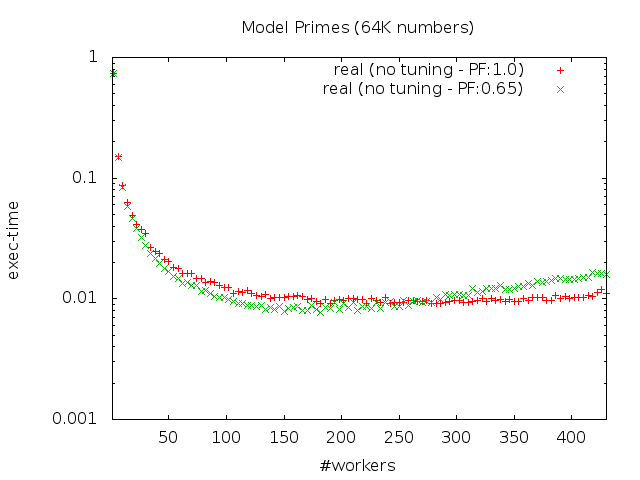
\includegraphics[width=0.55\paperwidth]{../BPG/images/MWfeatures-model.png}
	\caption{Real application execution time for partition factor values 1.0 and 0.65.}
	\label{fig:MWprimes-exhaustive}
\end{figure}

\begin {comment}

\paragraph{Best practice for choosing the initial number of workers}\label{para:mw-choose}\mbox{}\\

The results so far demonstrate that the analytical models implemented in the Master-Worker plugin produce quite accurate results. However, it can be statistically demonstrated that the partition factor estimated to balance the application for a certain number of workers is likely to be invalid if the number of workers changes significantly. This effect could be particularly adverse as the number of workers increases as load imbalances can reappear.

We will follow the case presented in the previous section to exemplify this issue and to show how to correct it. The plugin has estimated a partition factor of 0.65 to balance the application for 10 workers and it has subsequently estimated that the application can exploit 188 workers efficiently. This is a significant change from 178 workers {\color{red} Comment from ML: "178 workers? - where has this been mentioned before??" }   and, consequently, it is likely that the partition factor of 0.65 will not achieve good load balancing for this number of workers. This effect can be appreciated in Figure \ref{fig:MWprimes-exhaustive} because, even though the minimum execution time is obtained for 186 workers, the number of workers that are efficiently used should be approximately 150 workers. The best practice to correct this deviation is to execute PTF again, but using as the initial number of workers the results obtained in the first execution (206 in the example).  {\color{red} Comment from ML: "but using as the initial number of workers the results obtained in the first execution (206 in the example" - this is confusing - what is meant here?}

In this case, the first tuning step will produce the estimation shown in Table \ref{tab:mw-pf-estimation-206} for different values of the partition factor. This time, the plugin chooses 0.6 as the best partition factor. Next, the plugin estimates that the best number of workers in this case is 219 and generates the nine scenarios shown in Table \ref{tab:mw-plug-res-206} (along with the execution time of each scenario).

\begin{table}
    \centering
    \begin{tabular}{|c | c|}
    \hline
 {Partition Factor} &{Estimated Execution Time}\\\hline\hline
 0.10 & 0.01699\\
0.15 & 0.01677\\
0.20 & 0.01669\\
0.25 &  0.01662\\
0.30 & 0.01657\\
0.35 &  0.01653\\
0.40 &  0.01651\\
0.45 & 0.01649\\
0.50 & 0.01648\\
0.55 & 0.01645\\
0.60 & 0.01642\\
0.65 & 0.01644\\
0.70 & 0.01650\\
0.75 & 0.01671\\
0.80 & 0.01689\\
0.85 & 0.01709\\
0.90 & 0.01696\\
0.95 & 0.01762\\\hline
    \end{tabular}
    \caption{Estimation of the application execution time using 206 workers for different values of the partition factor.}
\label{tab:mw-pf-estimation-206}
\end{table}

Based on these results, the Master-Worker plugin advises the user to choose a partition factor of 0.54 and 240 workers. This advice is reliable as the means to reduce the imbalance when using more workers is to reduce the partition factor. Figure \ref{fig:MWprimes-exhaustive-206} shows the execution time of the application using a partition factor of 1.0, 0.65 and 0.54, respectively, in the range 4 to 430 workers. It can be seen that using a partition factor of 0.54 reduces the execution time of the application even more, and that the best time is obtained with 238 workers.

\begin{table}
    \centering
    \begin{tabular}{|c | c| c| c|}
    \hline
 {Scenario} &{Execution Time}& {Partition Factor} & {Number of Workers} \\\hline\hline
0  & 0.05506 & 0.54  & 198\\
1  & 0.05137 & 0.54  & 219\\
2  &  0.04966 & 0.54  & 240\\
3  & 0.05251 & 0.60  & 198\\
4  & 0.05553 & 0.60 & 219\\
5  &  0.05315 & 0.60 & 240\\
6  &  0.05410 & 0.66 & 198\\
7  & 0.05363 & 0.66 & 219\\
8  & 0.05200 & 0.66 & 240\\\hline
    \end{tabular}
    \caption{Results for the plugin generated scenarios.}
\label{tab:mw-plug-res-206}
\end{table}

Summarizing, if the tuning process with PTF advises a number of workers which is significantly larger than the one used to estimate the partition factor (the one indicated by the user in the execution command) then repeating the experiment using the advised number of workers will likely produce a better combination of the tuning parameters.

\begin{figure}[bt]
  \center
  \includegraphics[width=0.55\paperwidth]{../BPG/images/MWfeatures-model-206.png}
	\caption{Real application execution time for partition factor values 1.0, 0.65 and 0.54.}
	\label{fig:MWprimes-exhaustive-206}
\end{figure}
\end{comment}


\subsubsection{Uninstrumented applications supported for number of workers}\label{para:mw-unints}

The Master-Worker plugin cannot use analytical models for estimating the partition factor and number of workers if the application is not instrumented or it does not include a partition factor variable in its source code.  However, the plugin includes the possibility of tuning only the number of workers using an exhaustive search strategy. In this case, the user can just specify the range of workers and the step of the search. For example, the forest fire propagation application S2F2M \cite{Mostaccio05}  does not include a mechanism for load balancing (partition factor). In this case, we specify the range of 32 to 192 workers with step 4. The results obtained by PTF are shown in Table \ref{tab:mw-plug-res-s2f2m}, where it can be seen that the plugin advises the user to choose 176 workers (scenario 36).

\begin{table}
    \centering
    \begin{tabular}{|c | c| c|}
    \hline
 {Scenario} &{Execution Time}& {Number of Workers} \\\hline\hline
0	&	53.376	&	32	\\
1	&	47.975	&	36	\\
2	&	43.410	&	40	\\
3	&	39.664	&	44	\\
4	&	36.662	&	48	\\
5	&	34.372	&	52	\\
%6	&	32.206	&	56	\\
%7	&	30.237	&	60	\\
%8	&	28.815	&	64	\\
%9	&	27.479	&	68	\\
%10	&	26.202	&	72	\\
%11	&	25.220	&	76	\\
%12	&	24.361	&	80	\\
%13	&	23.516	&	84	\\
%14	&	22.545	&	88	\\
%15	&	21.873	&	92	\\
%16	&	21.132	&	96	\\
%17	&	20.664	&	100	\\
%18	&	19.933	&	104	\\
%19	&	19.581	&	108	\\
%20	&	19.119	&	112	\\
%21	&	19.453	&	116	\\
%22	&	18.357	&	120	\\
...	&	...		&	...	\\
%23	&	17.901	&	124	\\
%24	&	18.127	&	128	\\
%25	&	18.151	&	132	\\
%26	&	18.227	&	136	\\
27	&	19.196	&	140	\\
28	&	19.428	&	144	\\
29	&	17.815	&	148	\\
30	&	17.361	&	152	\\
31	&	18.008	&	156	\\
32	&	17.069	&	160	\\
33	&	17.520	&	164	\\
34	&	17.940	&	168	\\
35	&	17.374	&	172	\\
36	&	15.983	&	176	\\
37	&	17.337	&	180	\\
38	&	17.213	&	184	\\
39	&	16.546	&	188	\\
40	&	17.181	&	192	\\\hline
    \end{tabular}
    \caption{Results for the plugin generated scenarios.}
\label{tab:mw-plug-res-s2f2m}
\end{table}





\clearpage

\subsection{MPI Parameters Plugin}
%Contents of the plugin features section of D5.5
In order to guide the user on how best to exploit certain features of the MPI Parameters Plugin we will focus on the the Fish School Simulator application (FSSIM) \cite{Mostaccio05}.

\subsubsection{Multiple MPI flavors}\label{para:MPI-mult}

The MPI Parameters plugin offers some degree of support for three different implementations of  MPI: IBM MPI, Intel MPI and OpenMPI. In these cases, the keywords {\tt ibm}, {\tt intel}, or {\tt openmpi} should appear at the beginning of the configuration file.  Then, the plugin interprets that the user is specifying command line options and modifies the application execution command accordingly to the syntax established by the specific implementation.

Assuming that the user has included the parameter for tuning the eager limit in the configuration file, the MPI Parameters plugin will, for example, generate the following command line in each case:

\begin {itemize}
\item IBM MPI: mpiexec -n 64 executable -eager\_limit 16384
\item Intel MPI: mpiexec -genv I\_MPI\_EAGER\_THRESHOLD 16384 -n 64 executable
\item OpenMPI: mpiexec -mca osc\_pt2pt\_eager\_limit 16384 -n 64 executable
\end{itemize}

In any other case, the plugin interprets that the parameters indicated by the user are environment variables and produces the corresponding export commands before re-executing the application.  In addition, three example configuration files are provided along with the MPI Parameters plugin, one for each supported implementation (Intel MPI, IBM MPI and OpenMPI). They can be used as a quite complete starting point for tuning a rich set of MPI parameters. However, the user can also modify them (eliminating, adding or changing parameters) with the objective of fitting them to a particular application.

The three configuration files included with the PTF release are the following:

\begin {enumerate}
\item IBM MPI

\begin{verbatim}
MPIPO_BEGIN ibm
eager_limit=4096:2048:65560;
buffer_mem=8388608:2097152:134217728;
use_bulk_xfer=yes,no;
bulk_min_msg_size=4096:4096:1048576;
pe_affinity=yes,no;
cc_scratch_buf=yes,no;
wait_mode=nopoll,poll;
css_interrupt=yes,no;
polling_interval=100000:10000:1000000;
SEARCH=gde3;
MPIPO_END
\end{verbatim}

\item Intel MPI

\begin{verbatim}
MPIPO_BEGIN intel
I_MPI_EAGER_THRESHOLD=4096:2048:65560;
I_MPI_INTRANODE_EAGER_THRESHOLD=4096:2048:65560;
I_MPI_SHM_LMT=shm,direct,no;
I_MPI_SPIN_COUNT=1:2:500;
I_MPI_SCALABLE_OPTIMIZATION=yes,no;
I_MPI_WAIT_MODE=yes,no;
I_MPI_USE_DYNAMIC_CONNECTIONS=yes,no;
I_MPI_SHM_FBOX=yes,no;
I_MPI_SHM_FBOX_SIZE=2048:512:65472;
I_MPI_SHM_CELL_NUM=64:4:256;
I_MPI_SHM_CELL_SIZE=2048:1024:65472;
SEARCH=gde3;
MPIPO_END
\end{verbatim}

\item OpenMPI

\begin{verbatim}
MPIPO_BEGIN openmpi
mpi_paffinity_alone=0,1;
btl_openib_eager_limit=1024:2048:65560;
btl_openib_free_list_num=2:4:128;
btl_openib_use_eager_rdma=0,1;
btl_openib_eager_rdma_num=1:2:32;
btl_sm_eager_limit=1024:2048:65560;
btl_sm_num_fifos=1:1:10;
btl_sm_fifo_size=2048:512:65472;
btl_sm_free_list_num=2:4:128;
MPIPO_END
\end{verbatim}
\end {enumerate}

\subsubsection{Genetic search}\label{para:MPI-gen}

PTF has been enriched with the implementation of a search strategy based on the \textit{Generalized Differential Evolution 3 (GDE3)} genetic algorithm. In this strategy a population of ten initial scenarios is randomly generated and executed, then, an iterative process is followed, generating new populations by selecting the best five scenarios (those with the smallest execution time) for the next generation (elitism), generating five new scenarios by crossing over the previous population (crossover), and introducing mutations with a fixed probability (mutation). The number of iterations can be configured, but, generally, a close to optimal solution can be found in less than 30 iterations (generations).

For our use cases we have used a medium size population of fishes (64K), to avoid long executions, and have run the MPI application on 64 compute cores. In addition, given that it is not possible to test a large set of parameters combinations exhaustively in a reasonable time, we have used the exhaustive search strategy for a very limited configuration (see Table \ref{table:MPIConfigFileExhaustive}) of the parameters, and the heuristic search strategy for a more complete configuration (see Table \ref{table:MPIConfigFileGDE3}).

\begin{table}[tb]
	\centering
	\begin{footnotesize}
		\begin{tabular}{| l | }
		\hline
			\\
			MPI\_PIPO BEGIN ibm \\
			eager\_limit=4096:15366:65560; \\
			use\_bulk\_xfer=yes,no; \\
			bulk\_min\_msg\_size=4096:4096:1048576; \\
			task\_affinity=CORE,MCM; \\
			pe\_affinity=yes,no; \\
			cc\_scratch\_buf=yes,no; \\
			MPI\_PIPO END \\
			\\
		\hline
		\end{tabular}
	\caption{Configuration file for the exhaustive search.}
	\label{table:MPIConfigFileExhaustive}
	\end{footnotesize}
\end{table}


\begin{table}[tb]
	\centering
	\begin{footnotesize}
		\begin{tabular}{| l | }
		\hline
			\\
			MPIPO\_BEGIN ibm\\
			eager\_limit=4096:2048:65560;\\
			buffer\_mem=8388608:2097152:134217728;\\
			use\_bulk\_xfer=yes,no;\\
			bulk\_min\_msg\_size=4096:4096:1048576;\\
			cc\_scratch\_buf=yes,no;\\
			wait\_mode=nopoll,poll;\\
			css\_interrupt=yes,no;\\
			polling\_interval=100000:10000:1000000;\\
			task\_affinity=CORE,MCM; \\
			pe\_affinity=yes,no; \\
			SEARCH=gde3; \\
			MPI\_PIPO END \\
			\\
		\hline
		\end{tabular}
	\caption{Configuration file for the GDE3 search.}
	\label{table:MPIConfigFileGDE3}
	\end{footnotesize}
\end{table}


The exhaustive search strategy generates all possible combinations of the selected parameters and values, 320 in our example. Each scenario is executed and the one with the smallest wall time is chosen as the best one. The best combination corresponds to scenario 217: {\tt use\_bulk\_xfer} yes, {\tt bulk\_min\_msg\_size} 796672, {\tt cc\_scratch\_buf} no, {\tt task\_affinity} CORE, {\tt eager\_limit} 50194, {\tt pe\_affinity} yes. The execution time for this scenario was 2.8 sec, which is 1.6 times better than the time for the execution using the parameters default values (4.4 sec). The drawback is that for finding the optimal scenario in the set of tested ones, PTF needed 21505.2 sec (almost 6 hours) for the use case here.

The genetic search strategy (GDE3) can also be used for the same tuning space, but can even handle much larger tuning spaces consisting of significantly more parameters and possible values. For the use case we provide here, it executes 20 different scenarios in 1138.65 sec (approximately 20 min), which reduces the analysis time by a factor of 19 with respect to the exhaustive search. The best scenario in this case was found to be number 14: {\tt use\_bulk\_xfer} no, {\tt bulk\_min\_msg\_size} 988789, {\tt css\_interrupt} no, {\tt wait\_mode} poll, {\tt polling\_interval} 636027, {\tt cc\_scratch\_buf} no, {\tt task\_affinity} CORE, {\tt buffer\_mem} 102205313, {\tt eager\_limit} 59434, {\tt pe\_affinity} yes. The execution time for this scenario was 2.8 sec, again significantly better than the one obtained with the default values and now the search time has also been significantly reduced.  These results demonstrate that using the genetic search strategy can lead to results that are almost as good as the ones produced by the exhaustive search in only a fraction of the time needed for the latter.

\subsubsection{Eager-limit parameter strategy}\label{para:MPI-gen}

The MPI Parameters plugin includes an automatic strategy for determining if it is worthy to include the eager limit and memory buffer parameters into the plugin search space. Moreover, if it determines that it is worthy to include these parameters in the search, it will automatically generate the range of values that should be searched, trying to shrink this range in order to reduce the size of the search space. For using this strategy, the user only has to specify in the configuration file the option {\tt AUTO\_EAGER\_LIMIT=<eager-limit parameter>,<buffer-mem parameter>}. In our case, using IBM MPI, the configuration option is {\tt AUTO\_EAGER\_LIMIT=eager\_limit, buffer\_mem;}.

Here we test the plugin using this configuration option, where the FSSIM application was executed with a medium size population of 64K fishes and on 64 cores. The plugin determines that it is worthy to include the {\tt eager\_limit} and {\tt buffer\_mem} parameters into the search space because the total number of bytes communicated in point-to-point messages smaller than 64Kb was found to be greater than 30\% of the total number of bytes communicated in point-to-point messages. In addition, the plugin determines that the search range for the eager limit parameter should be between 1Kb and 32Kb because more than 80\% of the messages sent eagerly were in this range. Finally, the plugin uses the values determined for the eager limit and expression \ref{eqn:mem_buff} to compute the range for the buffer mem parameter range (128Kb to 4Mb).

\begin{equation}
	mem\_buff = 2{n}*{max(eager\_limit,64)}
\label{eqn:mem_buff}
\end{equation}

\begin{figure}[bth]
  \center
  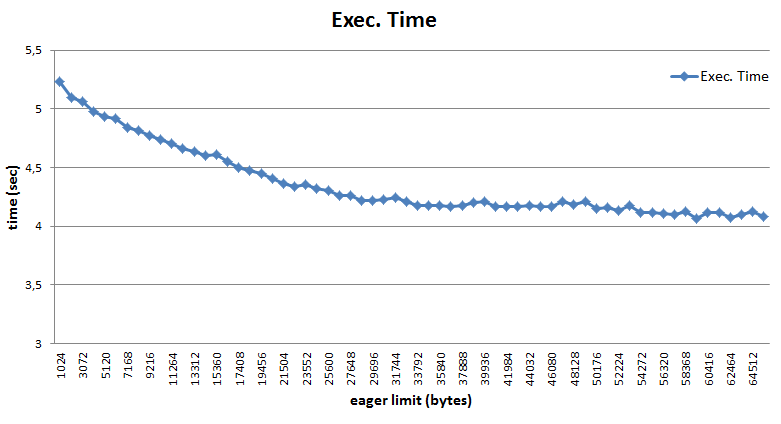
\includegraphics[width=0.65\paperwidth]{../BPG/images/MPIFssimEager.png}
	\caption{FSSIM execution time for different values of the eager limit and memory buffer parameters (IBM MPI).}
	\label{fig:fssimEager}
\end{figure}

\begin{figure}[bth]
  \center
  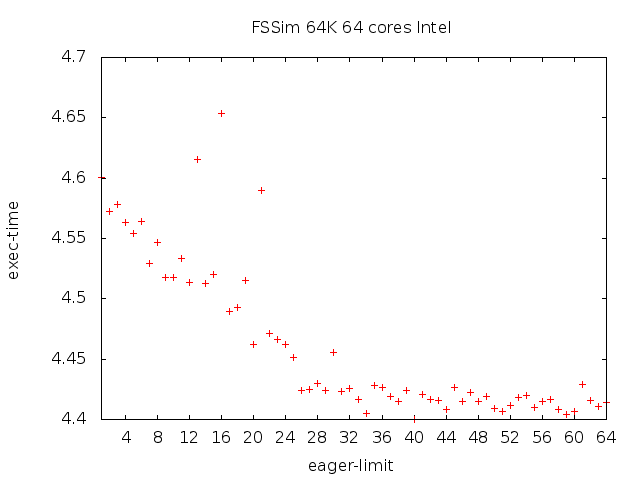
\includegraphics[width=0.65\paperwidth]{../BPG/images/MPImanual64cpu64kf.png}
	\caption{FSSIM execution time for different values of the eager limit and memory buffers parameters (Intel MPI).}
	\label{fig:fssimEagerIntel}
\end{figure}

Figures \ref{fig:fssimEager} and \ref{fig:fssimEagerIntel} clearly show that increasing the eager limit for this application up to approximately 30Kb produces  significant performance improvements, and that beyond this size no extra gains are obtained. This demonstrates that the eager limit strategy is successfully identifying the range of values that should be explored by the user for finding the best value for this parameter.


\clearpage


\clearpage

\bibliography{References}{}
\bibliographystyle{plainnat}

\end{document}
